\documentclass[12pt,a4paper]{book}
\usepackage[utf8]{inputenc}
%\usepackage[T1]{fontenc}
\usepackage{amsthm}
\usepackage{amsmath}
\usepackage{amsfonts}
\usepackage{amssymb}
\usepackage{graphicx}
\usepackage{physics}
\usepackage{cite}
\usepackage{caption}
\usepackage{subcaption}
%\usepackage{hyperref}
\usepackage{comment}
\usepackage{epsfig}
\usepackage{latexsym}
\usepackage{color} 
\usepackage{todonotes}
\usepackage{wrapfig}
\theoremstyle{definition}
\newtheorem{definition}{Definition}[section]
\newtheorem{theorem}{Theorem}[section]
\newtheorem{lemma}[theorem]{Lemma}

\linespread{1.2}
\usepackage[a4paper,top=2.5cm,bottom=2.5cm,left=3cm,right=2.5cm]{geometry}
\setlength{\marginparwidth}{2cm}
\title{Thesis Work: Ergotropy and Quantum Phase Transitions }
\author{}
\begin{document}
   \maketitle
\tableofcontents{}

   
\chapter{Introduction}
--------------------------------\\
Here go motivations and outline of the work, maybe something on quantum batteries  \cite{PhysRevE.87.042123} \cite{PhysRevB.99.205437} \cite{deffner2019quantum}, quantum machines, work extraction processes, quantum computers.\\
Also something on DMRG and Tensor Networks.\\
---------------------------------\\
We will define the ergotropy and some related quantities and study their behavior in a system that undergoes a quantum phase transition.\\
We will also define and measure a quantity related to ergotropy: the Max-Ergotropy.\\
Besides the interest of these quantities for experimental aspects related to work extraction, we will use them as quantum phase transition markers.\\
Entanglement plays a role, maybe focus on difference between classical and quantum work extraction.\\


---------------------------------\\


In the last decades, Quantum Phase Transitions (QPT) \cite{sachdev_2011} \cite{Vojta_2003}  established as one of the most important research topics in theoretical and experimental \cite{Baumann2010} condensed matter physics. \\
QPT appear in many areas of modern research: rare-earth magnetic insulators , heavy-fermion
compounds, high-temperature superconductors, two-dimensional
electron gases,  quantum Hall effects.\\
A lot of work has been done to understand what happens to the quantum wave-function that undergoes a Quantum Phase Transition.\\
The work of Wen et. al exploited the limitation of the symmetry breaking approach in the description of QPT  \cite{Xiao:803748}. Topological transitions and the distinction between Long-Range and Short-Range quantum entanglement pushed in the direction of a unification between Quantum Information and Quantum Matter. \cite{Zeng2019}\\
Following the incredible development of Quantum Information Theory  \cite{NielsChuang} \cite{wilde_2013}, it became clear that entanglement is a fundamental resource for the development of  Quantum Technology and entanglement measures gained a renew interest.\\ 
In 2002 \cite{Osterloh2002} Fazio et al. and  \cite{PhysRevA.66.032110} Nielsen et al. showed that Concurrence is sensible to QPT. \\
In 2008, Amico, Fazio, Osterloh and Vedral published a monumental review \cite{RevModPhys.80.517} on the topic of "Entanglement in Many-Body Systems" where they reviewed many entanglement measures and their role in QPT.  \\
A clear and complete characterization of quantum correlations in QPT it's still  an open problem \cite{De_Chiara_2018} even if by now it's clear that the various measures of entanglement
are sensitive to the presence of quantum
phase transitions. \cite{PhysRevLett.93.250404} \\ \todo{Here i cite various measures}
Various entanglement measures have been studied close to a QPT:
  Local Convertibility \cite{Franchini_2014},Quantum Discord \cite{Tomasello_2011}, Leggett-Garg
  inequalities\cite{PhysRevB.93.035441}. \\ 
 
Modern nanotechnology allows 
for testing concepts derived from classical thermodynamics
in regimes where quantum effects become crucial  \cite{PhysRevX.7.031044} \cite{Rossnagel_2016} \cite{Scully862}.\\
Quantum Thermodynamics \cite{Gemmer2010} \cite{deffner2019quantum} is a relatively new field that aims to characterize the Thermodynamics aspect of Quantum Many-Body Theory and the emergence of classical Thermodynamic from Quantum Mechanics. \\
Following this goal, Allahverdyan et al. \cite{allahverdyan2004maximal}  defined a quantity called ergotropy to solve the work extraction problem in the quantum regime.\\
Ergotropy for finite system becomes the Free Energy, the deviation of Ergotropy from is classical counterpart is proportional to quantum effects like entanglement and coherence \cite{PhysRevA.99.052320} \cite{Francica2017} and this difference could be crucial in the development of quantum technologies  \cite{PhysRevE.87.042123} .\\
Since ergotropy is sensible to quantum correlations, we believe it would be interesting to characterize it in the proximity of a  Quantum Phase Transition.

\clearpage


\chapter{Ergotropy and related measures}\label{sec:measures}
A very practical question we can ask ourselves is: If someone gives us a quantum mechanical system in a given state, what is the maximum amount of work we can extract from it?\\ 
This question becomes more meaningful if we restrict the ways in which we can modify the state.\\
A natural restriction we can set is that we want to use unitary channels only.\\
With this hypothesis in mind, the answer to this question exist and it is a quantity called \textit{ergotropy}
\cite{allahverdyan2004maximal}.\\
\section{Ergotropy}
We will follow the derivation in \cite{allahverdyan2004maximal}.\\
Consider a quantum mechanical system S described by an Hamiltonian $H$ on which we can act on with an external potential $V(t)$. \\
Examples could be:  \todo{should i give some examples?} \\
The state $\rho(t)$ of the system will thus evolve through the Hamiltonian: $H_{tot}=H+V(t)$ according to the Heisenberg equation: 
\begin{equation}\label{eq:heisen}
i \hbar \dot{\rho}(t)=[H_{tot}(t), \rho(t)]
\end{equation}
Defining the Unitary time-evolution operator $U(t) = \exp(iH_{tot}t/\hbar)$, we can write :
\begin{equation}\label{eq:time_evol}
	\rho(t)=U(t)\rho(0) U^\dagger(t)
\end{equation} 
Suppose now that the external potential is turned on in the time interval between $t=0$ and $t=\tau$, the total work done on the system will be:
\begin{equation}
	W=E(\tau)-E(0)=\tr[\rho(\tau) H]-\tr[\rho(0) H]
\end{equation}
If we want to extract the maximum amount of work from the system we have to reach a $\rho(\tau)$ such that $E(\tau)$ has the lowest possible value.\\
\begin{definition}[Passive State]\label{eq:def_passivestate} \cite{pusz1978}\\
Given an Hilbert Space with an Hamiltonian $H$, a state $\rho_{pas}$ is a passive state if:
	 \begin{equation}
		\tr[H \rho_{pas}] \leq \tr\left[H U \rho_{pas} U^{\dagger}\right] \quad \forall U \quad \text{with} \quad U U^\dagger=U^\dagger U = I
	\end{equation}
That means we can't lower the energy (and eventually extract work) from a Passive State acting on it with Unitary Matrices.
\end{definition}
Putting all together: we would like to find a function $V_{pas}(t)$, which is zero outside of the time interval $[0,\tau]$, such that the Hamiltonian $H_{pas}=H+V_{pas}(t)$ acting on the system trough the time-evolution operator $U_{pas}(t) = \exp(iH_{pas}t/\hbar)$ will transform the state $\rho(0)$ in the passive state $\rho_{pas}$ that has energy:
\begin{equation}
	 E_{pas}=\tr[ \rho_{pas}H]=\tr[U_{pas}(\tau)\rho(0)U_{pas}^\dagger(\tau) H]
\end{equation}
And $E_{pas}$ will be the lowest energy we can get using unitary operators.\\
Acting with unitary transformations only we can't change the eigenvalues of $\rho(0)$, nevertheless we can reach a passive state. \\ Let's first prove the following  \cite{harrell2013course}:
\begin{theorem}\label{theo:passive}
Given an Hilbert Space with Hamiltonian 
\begin{equation}
	H=\sum_{k \geq 1} \varepsilon_{k}^{(\uparrow)}\ket{\varepsilon_{k}^{(\uparrow)}}\bra{\varepsilon_{k}^{(\uparrow)}} \quad \text{with} \quad \varepsilon_{1}^{(\uparrow)} \leq \varepsilon_{2}^{(\uparrow)} \leq \cdots
\end{equation}
and a generic quantum state:
\begin{equation}
	\rho=\sum_{j \geq 1} r_{j}^{(\downarrow)}\left|r_{j}^{(\downarrow)}\right\rangle\left\langle r_{j}^{(\downarrow)}\right| \quad \text{with} \quad  r_{1}^{(\downarrow)} \geq r_{2}^{(\downarrow)} \geq \cdots
\end{equation}
The state:
\begin{equation}\label{eq:rhopas}
	\rho_{pas}=\sum_{j} r_{j}^{(\downarrow)}\ket{\varepsilon_{j}^{(\uparrow)}}\bra{\varepsilon_{j}^{(\uparrow)}}
\end{equation}
is a passive state.
\end{theorem}

\begin{proof}
We represent a generic unitary matrix in the Hamiltonian basis \footnote{If the basis it's not complete we can easily expand it setting the new eigenvalues to 0.}:
\begin{equation}
 	U=\sum_{j}U_{ij}\ket{\varepsilon_{i}}\bra{\varepsilon_{j}}
\end{equation}
Since $U$ it's unitary, $|U_{ij}|^2$ is a doubly stochastic matrix (has non-negative entries and each row and column sums to 1), that means we can use the Birkhoff’s Theorem \cite{marshall11} to express it as a convex combination of permutation matrices $P^n$:
\begin{equation} 
	|U_{ij}|^2=\sum_{n} p_{n} P^{n} \quad \text{with} \quad \sum_{n} p_{n} = 1 
\end{equation}
Now we apply this generic unitary transformation $U$ to $\rho_{pas}$ and calculate the resulting energy:
\begin{equation}
	\tr[U \rho_{pass}U^{\dagger} H ]=\sum_{i, k} \varepsilon_{i}^{(\uparrow)} r_{k}^{(\downarrow)}\left\|U_{i k}\right\|^{2}=\sum_{n}p_n \sum_{i, k}\varepsilon_{i}^{(\uparrow)} P^n_{ik}  r_{k}^{(\downarrow)}
\end{equation}
For every permutation $P(r_{j}^{(\downarrow)})$  of the $\rho_{pass}$ indices it's clear that:
\begin{equation}
	\sum_{i}\varepsilon_{i}^{(\uparrow)}[P(r_{j}^{(\downarrow)})]_i \geq \sum_{i}\varepsilon_{i}^{(\uparrow)} r_{i}^{(\downarrow)}=\tr[\rho_{pas}H]
\end{equation}
the permutation that gives us the lowest product is the one where the eigenvalues are arranged in the opposite direction.\\
We conclude that:
\begin{equation}
\sum_{n}p_n \sum_{i, k}\varepsilon_{i}^{(\uparrow)} P^n_{ik}  r_{k}^{(\downarrow)} \ge \sum_{n}p_n \sum_{i}\varepsilon_{i}^{(\uparrow)} r_{i}^{(\downarrow)}=\sum_{i}\varepsilon_{i}^{(\uparrow)} r_{i}^{(\downarrow)}
\end{equation}
Or equivalently:
\begin{equation}
	\tr [\rho_{pas} H]\leq \tr[U \rho_{pass}U^{\dagger} H ] \quad \forall U \quad \text{with} \quad U U^\dagger=U^\dagger U = I
\end{equation}
\end{proof}
We proved that from  every quantum state 	$\rho=\sum_{j \geq 1}  r_{j}^{(\downarrow)}\left|r_{j}\right\rangle\left\langle r_{j}\right| $ we can form a passive state	$\rho_{pas}=\sum_{j} r_{j}^{(\downarrow)}\left|\varepsilon_{j}\right\rangle\left\langle\varepsilon_{j}\right|$, it remains only to show that we can go from $\rho$ to $\rho_{pas}$ with an appropriate choice of the function $V(t)$.\\
An unitary operator that does the job is: 
\begin{equation}\label{eq:upas}
	U_{pas}=\sum_{j}\left|\varepsilon_{j}\right\rangle\left\langle r_{j}\right|
\end{equation}

\begin{comment}
In this picture the Heisenberg equation () becomes:
\begin{equation}
i \hbar \dot{\rho_I}(t)=[V_{I}(t), \rho_I(t)]
\end{equation}
\end{comment}
Assuming that the system hamiltonian $H$ in $H_{tot}=H+V(t)$ (\ref{eq:heisen}) does not depend on time, it is convenient to switch into the interaction picture:
\begin{equation}
	V_I(t)=e^{i H t / \hbar}  V(t) e^{-i H t / \hbar}
\end{equation}
the evolution operator $U_I(t)$ obeys:
\begin{equation}\label{eq:U_interaction}
	i \hbar \frac{d U_{I}(t)}{d t}=V_I(t) U_{I}(t) \quad \text{with} \quad U_I(0)=1
\end{equation}
We want that at  $t=\tau$:
\begin{equation}
	U_{I}(\tau) = e^{i H \tau / \hbar} U_{pas}\equiv e^{-i \Lambda \tau / \hbar} \implies  U_I(\tau) \rho_I(0) U_I^\dagger(\tau)=\rho_I(\tau)=(\rho_{pas})_I
\end{equation}
Where the  $\Lambda$ matrix is obtained by diagonalization.\\
To achieve the desired $U_I$ with an interaction $V(t)$ we can define a simple function $\varphi(t)$  that respects the following conditions:
\begin{equation}\label{eq:phiconditions}
\varphi(0)=\dot{\varphi}(0)=\dot{\varphi}(\tau)=0 \quad \varphi(\tau)=\tau
\end{equation}
so that choosing as a potential:
\begin{equation}\label{eq:vpas}
	(V_{pas}(t))_I\equiv \dot{\varphi}(t)  \Lambda 
\end{equation}
The evolution operator will be (\ref{eq:U_interaction}):
\begin{equation}
	U_{I}(t)=e^{-i \Lambda \varphi(t) / \hbar}
\end{equation}
and because of the conditions ($\ref{eq:phiconditions}$) we imposed on $\varphi$:
\begin{equation}
	U_{I}(0)=1 \quad 	U_{I}(\tau) = e^{-i \Lambda \tau / \hbar}=e^{i H \tau / \hbar} U_{pas}
\end{equation}
and $V(0)=V(\tau)=0$.\\
We explained the notion of \textit{passive state} (def. \ref{eq:def_passivestate}) and we showed that with an appropriate choice of $V(t)$ (eq. \ref{eq:vpas}) we can transform a generic state into a passive one.\\
We are now ready to give a general definition of \textit{ergotropy}:
\begin{definition}[Ergotropy]\label{eq:def_ergotropy}
	The ergotropy is the maximum amount of work we can extract from a state $\rho$ using unitary operators:
\begin{equation}
	\mathcal{W}(\rho, H)\equiv max _{U}[\tr(\rho H)- \tr\left(U \rho U^{\dagger} H\right)]=\tr(\rho H)-\min _{U}\tr\left(U \rho U^{\dagger} H\right)
\end{equation}
\end{definition}
For our problem the unitary matrices are the time-evolution operators (eq. \ref{eq:time_evol}).\\
Using Th. \ref{theo:passive} and the procedure of eqs. \ref{eq:upas}- \ref{eq:vpas} we can saturate the ergotropy bound:
\begin{equation}\label{eq:ergowithpas}
	\mathcal{W}(\rho, H)=\tr(\rho H)-\min _{U}\tr\left(U \rho U^{\dagger} H\right)=\tr(\rho H)-\tr(\rho_{pas}H)
\end{equation}
With $\rho_{pas}(\rho,H) $ as in (eq. \ref{eq:rhopas}):
\begin{equation}
	\rho_{pas}=\sum_{j} r_{j}^{(\downarrow)}\ket{\varepsilon_{j}^{(\uparrow)}}\bra{\varepsilon_{j}^{(\uparrow)}}
\end{equation}
where as usual the eigenstates with the largest eigenvalues are the least energetic ones.


\todo{difference between ergotropy and classical exctractable work?}

\section{Max-Ergotropy}
Despite Ergotropy has a clear experimental meaning, its calculation is not numerically efficient. To see this
let's rewrite more explicitly eq. \ref{eq:ergowithpas} :
\begin{equation}
	\mathcal{W}(\rho,H)=E(\rho)-E(\rho_{pas})=\sum_{j, k} r_{j}^{(\downarrow)} \varepsilon_{k}^{(\uparrow)}\left( \left|\braket{r_j^{(\downarrow)}}{\varepsilon_{k}^{(\uparrow)}}\right|^2-\delta_{jk}\right)
\end{equation} 
In the calculation of Ergotropy we need both the eigenvalues and the eigenvectors of $\rho$ and $H$, while for other known measures like Entropy \ref{eq:Entropy} or Purity \ref{eq:Purity} \todo{fix ref} we only need the eigenvalues of the density matrix $\rho$.\\ 
To solve this issue we can define the anti-ergotropy as:
\begin{definition}[Anti-Ergotropy]\label{eq:def_antiergotropy}
	\begin{eqnarray}
		{\cal A}(\rho,H)  \equiv E({\rho}_{a-pas} ) - E({\rho})
		= \sum_{j, k} r_{j}^{(\uparrow)} \varepsilon_{k}^{(\uparrow)}\left( \delta_{jk}-\left|\braket{r_j^{(\uparrow)}}{\varepsilon_{k}^{(\uparrow)}}\right|^2\right)
	\end{eqnarray}
\end{definition}
Where 
$\rho_{a-pas}=\sum_{j} r_{j}^{(\uparrow)}\ket{\varepsilon_{j}^{(\uparrow)}}\bra{\varepsilon_{j}^{(\uparrow)}}$ is the most energetic state we can get acting with unitary operators on $\rho$, it's called an \textit{anti-passive} state because much like def. \eqref{eq:def_passivestate}:
\begin{equation}
	E({\rho}_{a-pas} )=\tr[H \rho_{a-pas}] \ge \tr\left[H U \rho_{a-pas} U^{\dagger}\right] \quad \forall U \quad \text{with} \quad U U^\dagger=U^\dagger U = I
\end{equation}
And we can get rid of $E(\rho)$ defining:
\begin{definition}[Max-Ergotropy]
	The Max-Ergotropy of a state $\rho$ given an Hamiltonian $H$ is the (positive) difference between the  Anti-Ergotropy (def. \ref{eq:def_antiergotropy}) and the Ergotropy (def.\ref{eq:def_ergotropy}) :
	\begin{equation}
		\begin{aligned}
		&{\cal M}(\rho,H)  \equiv {\cal A}(\rho,H) -\mathcal{W}(\rho,H) = E({\rho}_{a-pas} ) - E({\rho}_{pas})	= \\
		&\sum_{i} (r^{(\uparrow)}_i -r^{(\downarrow)}_i) \varepsilon^{(\uparrow)}_i 
		\end{aligned}
	\end{equation}
The Max-Ergotropy of a state $\rho$ is the maximum energy difference between any two states that are unitary connected to $\rho$. 
\end{definition}
Notice that the Max-Ergotropy depends only on the eigenvalues of $\rho$ and $H$ as we desired.


\section{Entanglement Measures}
For a pure bipartite state, the problem of quantifying entanglement is clearly solved by the Von Neumann Entropy of (either of) the reduced density.\\
For a generic mixed state, the problem is much more difficult and
a plethora of measures exist \cite{RevModPhys.80.517}.

\subsection{Entanglement Entropies}

\begin{definition}[Von Neumann Entropy]
 The Von Neumann Entropy of a density matrix $\rho$ is:
  \begin{equation}
	S(\rho)=-\tr\left(\rho \log \rho \right)
  \end{equation}
\end{definition}
\begin{figure}[h]
	\centering
	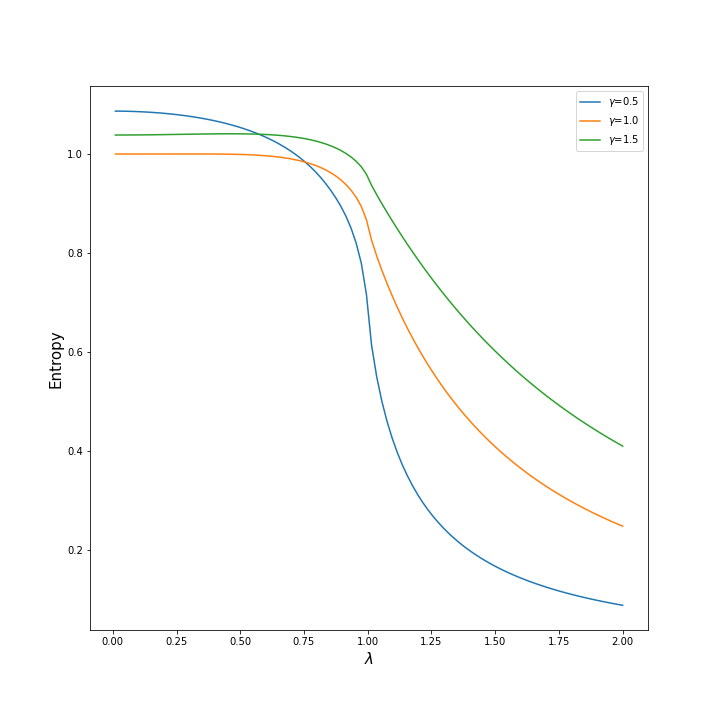
\includegraphics[width=0.7\linewidth]{graphs/entropy_3gammas}
	\caption{Analitical 2 site Von Neumann Entropy}
	\label{fig:entropy3gammas}
\end{figure}
\begin{figure}[h]
	\centering
	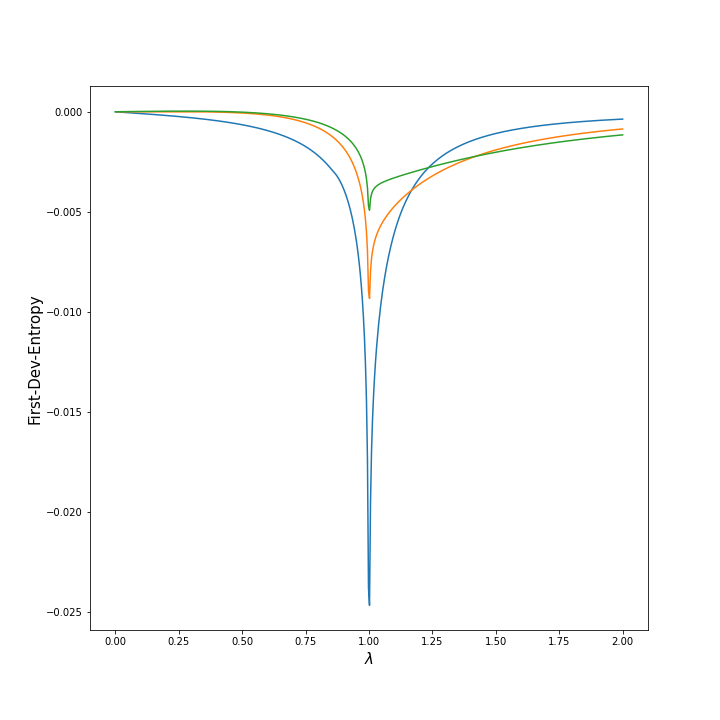
\includegraphics[width=0.7\linewidth]{graphs/firstdev_entropy_3gammas}
	\caption{Analitical 2 site first-dev Von Neumann entropy}
	\label{fig:firstdeventropy3gammas}
\end{figure}

\clearpage
\begin{definition}[Rényi entropy]
	The Rényi entropy of a density matrix $\rho$ is:

\end{definition}
\subsection{Concurrence}
\begin{definition}[Concurrence]
	The concurrence is defined only for a mixed state $\rho$ of two qubits (in our case the sites $i \  \text{and} \  j$ ) as :
\begin{equation}
	C(i, j)=\max \left\{0, r_{1}(i, j)-r_{2}(i, j)-r_{3}(i, j)-r_{4}(i, j)\right\}
\end{equation}
where $r_\alpha (i, j)$ are the square roots of the eigenvalues of the product matrix $R = \rho (i, j) \tilde{\rho} (i, j)$ and $\tilde{\rho}$ is obtained by a spin-flipping operation:
\begin{equation}
	\tilde{\rho} \equiv \sigma^{y} \otimes \sigma^{y} \rho^{*} \sigma^{y} \otimes \sigma^{y}
\end{equation}
\end{definition}
\cite{Osterloh2002} Fazio et al. and  \cite{PhysRevA.66.032110} Nielsen et al. studied the behavior of the concurrence $C(i, j)$ for an XY Model in the proximity of a quantum phase transition
\todo{Finite size study of Ergo?}
\begin{figure}[h]
	\centering
	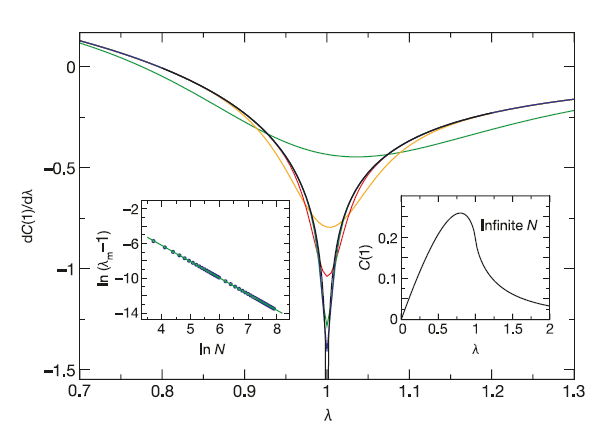
\includegraphics[width=0.7\linewidth]{graphs/osterlohfazio}
	\caption{First derivative of the concurrence $\partial_{\lambda}C$ in a  Ising Model the curves
		correspond to different lattice sizes: $N=11, 41, 101, 251, 401,\infty$. In the right inset is showed the concurrence for an infinite system. From \cite{Osterloh2002}}
	\label{fig:osterlohfazio}
\end{figure}\\
Redo fig. \ref{fig:nielsenconc} 
\begin{figure}[h]
	\centering
	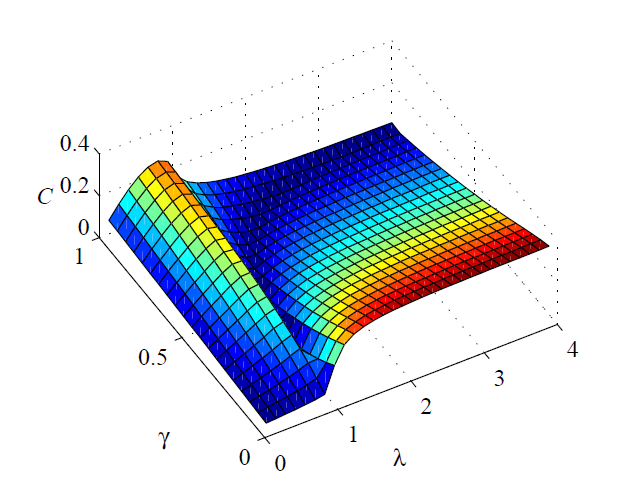
\includegraphics[width=0.7\linewidth]{graphs/nielsenconc}
	\caption{Analytical calculation, concurrence for the XY-model.where $\lambda=1/\lambda$ From \cite{PhysRevA.66.032110}}
	\label{fig:nielsenconc}
\end{figure}



\chapter{Quantum Phase Transitions}
The freezing of water or the magnetization of iron are some of the most famous phase transitions.\\
If we study the properties of a system for different values of the  thermodynamic variables we can draw a phase diagram \cite{Huang_1987} (fig. \ref{fig:phasediagramofwater}).

%\begin{wrapfigure}{r}{0.7\textwidth}
%	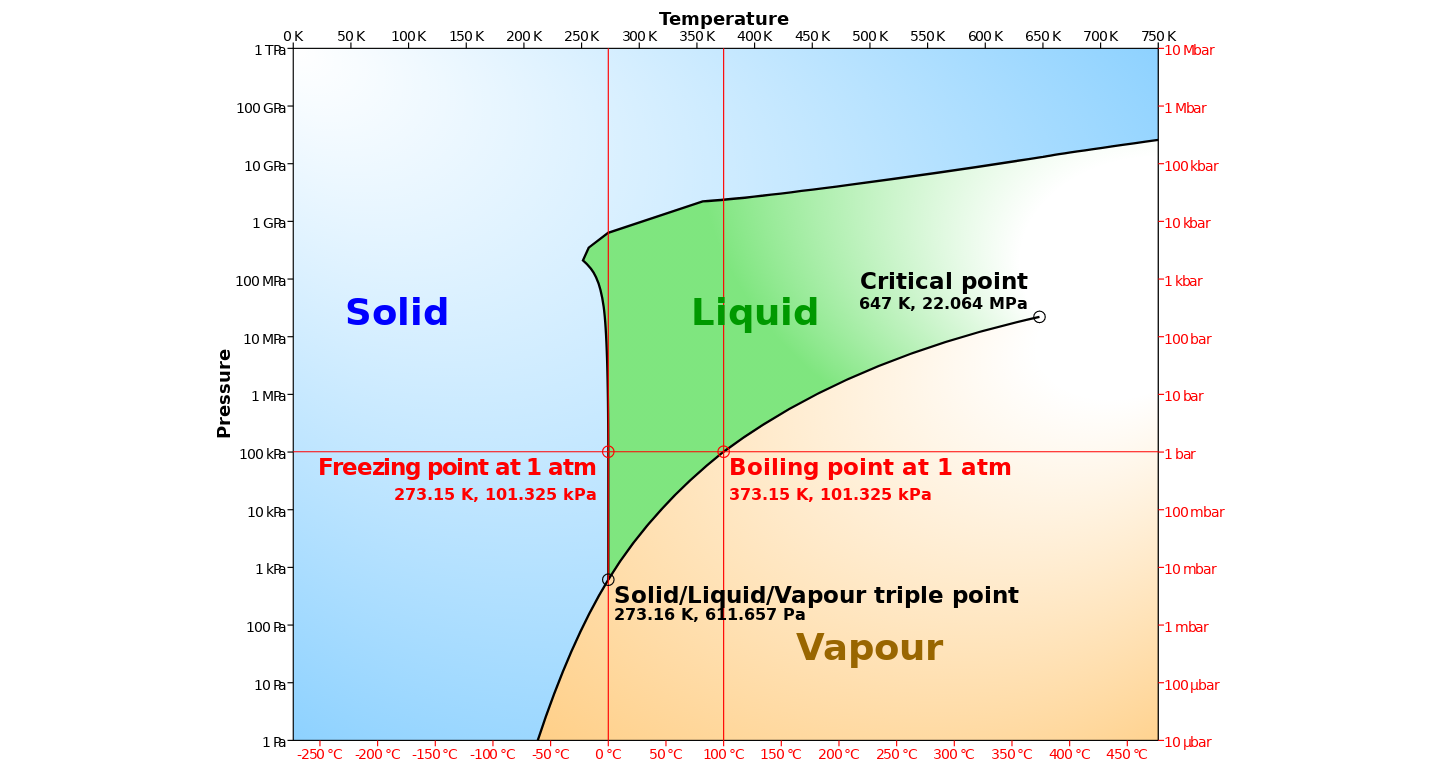
\includegraphics[width=\linewidth]{graphs/Phase_diagram_of_water}
%	\caption{Phase diagram of water}
%	\label{fig:phasediagramofwater}
%\end{wrapfigure}
\begin{figure}[h]
	\centering
	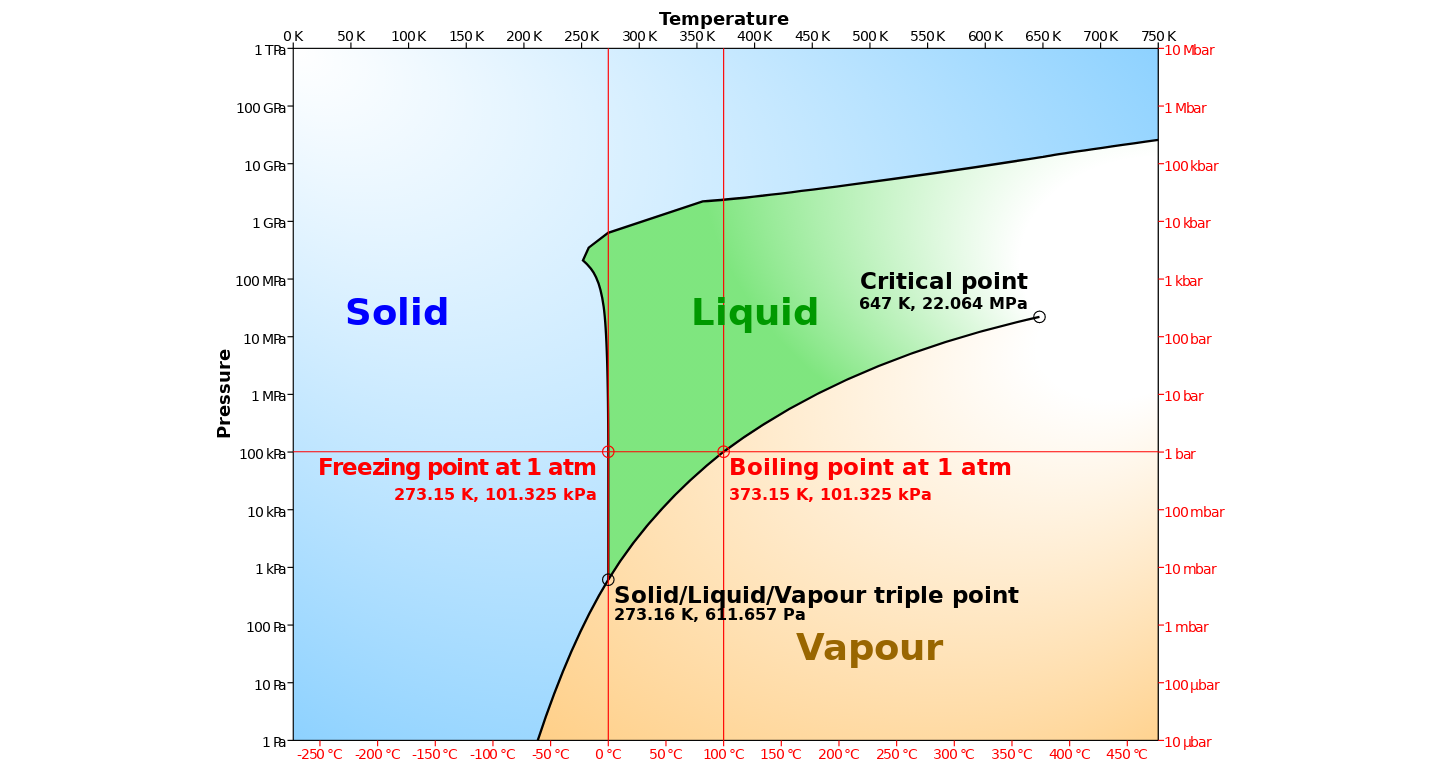
\includegraphics[width=0.7\linewidth]{graphs/Phase_diagram_of_water}
	\caption{Phase diagram of water, the solid lines represent the phase boundary. Note that the system can pass from liquid to vapour without experiencing a phase transition.}
	\label{fig:phasediagramofwater}
\end{figure}

The region of thermodynamic states where the macroscopic properties of the system are uniform it's called \textit{phase}.\\
Depending on the properties we are interested in, we can define for example the "solid phase" for water or the "ferromagnetic phase" for iron.\\
A \textit{phase transition} occurs when the system phase changes "abruptly".
The points where this phenomenon happens are called \textit{phase boundary}.\\
This "abrupt" change corresponds mathematically to a non-analytic behavior of some thermodynamic function \cite{Goldenfeld_1992}.\\ 
For classical thermodynamic systems, the standard function used to detect phase transitions is the free-energy.\\
A phase transition that occurs at $T=0$ is called a \textit{Quantum phase transition}.\cite{sachdev_2011}.\\
In a classical system at $T=0$ every particle is freezed in a completely motionless state : even theoretically a phase transition is impossible. On the other hand, in Quantum Mechanics, the Heisenberg uncertainty principle generates some fluctuations in the quantum state;
at sufficiently low temperatures, these fluctuations become relevant and can drive a phase transition.\\
Practically speaking, the quantum phase boundary correspond to non-analitical points in the ground-state energy of an infinite lattice system.\\ 
\begin{figure}[h]
	\centering
	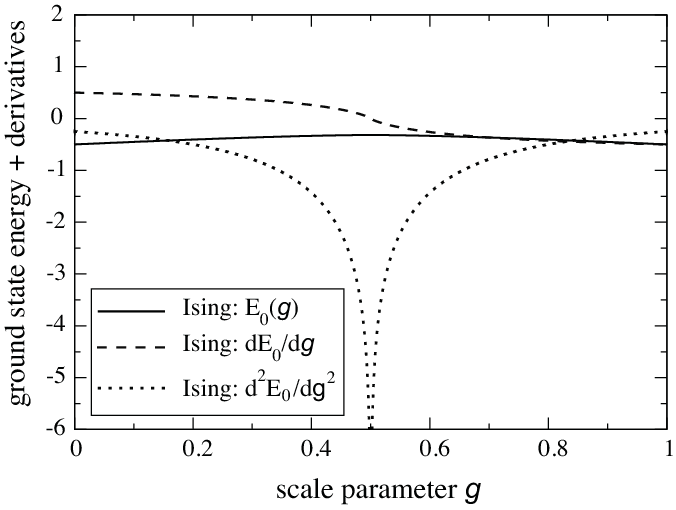
\includegraphics[width=0.7\linewidth]{graphs/divergence-ising-model}
	\caption{From \cite{PhysRevA.81.032305}: Ground state energy and derivatives of an Ising Model with a transition at $g=0.5$ }
	\label{fig:divergence-ising-model}
\end{figure}

\section{XY model}
The XY model in a transverse magnetic field it's one of the few integrable models to exhibits non trivial phases \cite{Franchini_2017}, in 1D it is described by the Hamiltonian:

\begin{equation}\label{eq:XYmodelHam}
	H_{X Y}=-\frac{1}{2} \sum_{l=1}^N\left(\frac{1+\gamma}{2} \sigma_{l}^{x} \sigma_{l+1}^{x}+\frac{1-\gamma}{2} \sigma_{l}^{y} \sigma_{l+1}^{y}+\lambda \sigma_{l}^{z}\right)
\end{equation}
On the l site lives a Spin-1/2 variable described by the 3 Pauli Matrices $\sigma_{l}^{x},\sigma_{l}^{y},\sigma_{l}^{z}$ , N is the total number of sites. \\ The Hamiltonian has 2 parameters:
$\lambda \in \mathbb{R}$ is the strength of the external magnetic field and $\gamma \in \mathbb{R}$ it's used to quantify the amount of anisotropy in the spin-spin interaction. \\
For $\gamma=1$ we have the well-known 1D Transverse-Field Ising Model (TFIM) while at $\gamma=0$ the Hamiltonian is the 1D XX model.\\
This model was solved for the first time by Lieb Schultz and Mattis
\cite{LIEB1961407} for $\lambda=0$, Katsura \cite{PhysRev.127.1508} solved it for $\lambda \ne 0$ and later Barouch and McCoy calculated the correlation functions on the ground state  \cite{barouch1} \cite{barouch2} \cite{barouch3}.\\
A rotation by $\pi/2$ along the z-axis interchanges the x and y spin interactions and is equivalent to 
 $\gamma \rightarrow -\gamma$
, while a reflection of the spin across the x-y plane is compensated by $h \rightarrow -h$: thus we will concentrate only on the first quadrant of the phase diagram $(\gamma \ge 0, \lambda \ge 0)$ .

\begin{figure}[h]
	\centering
	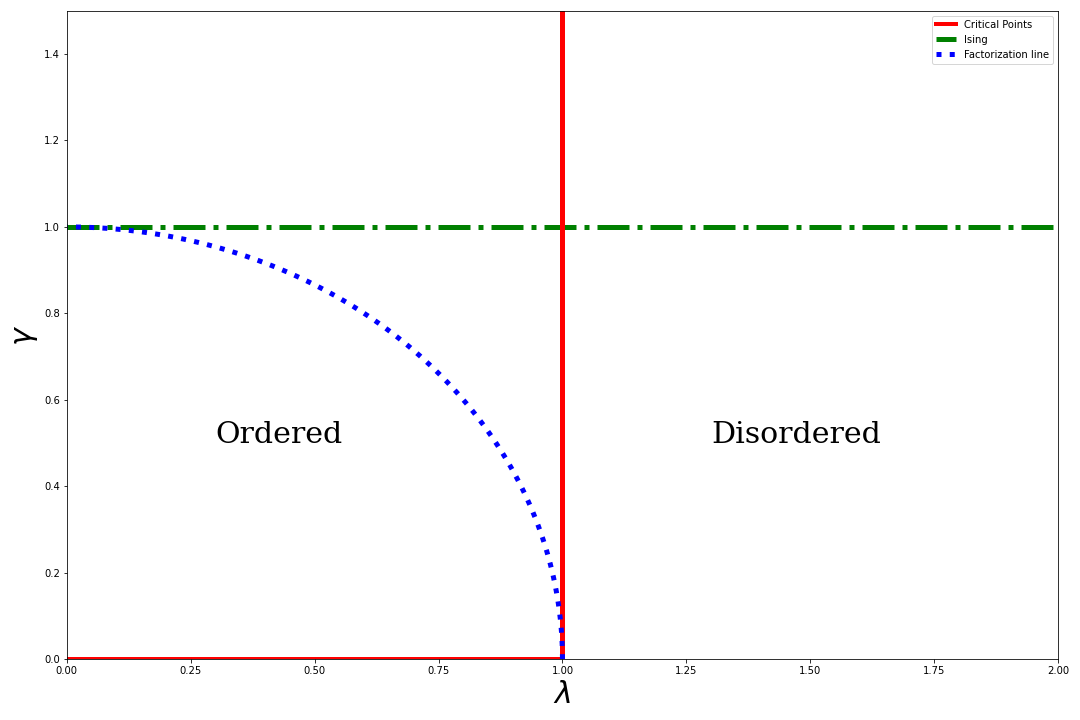
\includegraphics[width=0.7\linewidth]{graphs/xymodelphaseplot}
	\caption{Zero temperature phase diagram of the XY-Model. The phase boundary corresponds to the red line. For $\gamma^2+h^2=1$ the the ground state becomes a product state (blue dashed line). }
	\label{fig:phase-diagram-of-the-xy-model}
\end{figure}
For $\gamma>0$ we see that the critical line at $\lambda=1$ identifies two phases: the "ordered" or  \textit{ferromagnetic} phase and the "disordered" or \textit{paramagnetic} phase.\\

For $\lambda <1$ the interaction term (eq. \ref{eq:interactionterm}) dominates.
\begin{equation}\label{eq:interactionterm}
	H_{int}= -\frac{1}{2} \sum_{l=1}^N \left(\frac{1+\gamma}{2} \sigma_{l}^{x} \sigma_{l+1}^{x}+\frac{1-\gamma}{2} \sigma_{l}^{y} \sigma_{l+1}^{y} \right)
\end{equation}
The ground states are a combination of two states completely aligned in opposite directions (ferromagnetic states):
\begin{equation}
	\ket{\psi_g}=\alpha \ket{\rightarrow \rightarrow...\rightarrow} + \beta \ket{\leftarrow \leftarrow ... \leftarrow}
\end{equation} 
The ferromagnetic states are aligned in the x-direction if $\gamma>0$ and in the y-direction if $\gamma<0$.\\
In real systems with a large number of spins, $\ket{\psi_g}$ is never found in this quantum superposition: decoherence makes the system choose one of the two ordered states.\\
For $\lambda >>1$ there is only one ground state: $\ket{\uparrow \uparrow...\uparrow}$; due to this missing degeneracy, the system makes a transition from a gapless to a gapped ground-state (fig. \ref{fig:gapscaling}.\\
\begin{figure}[h]
	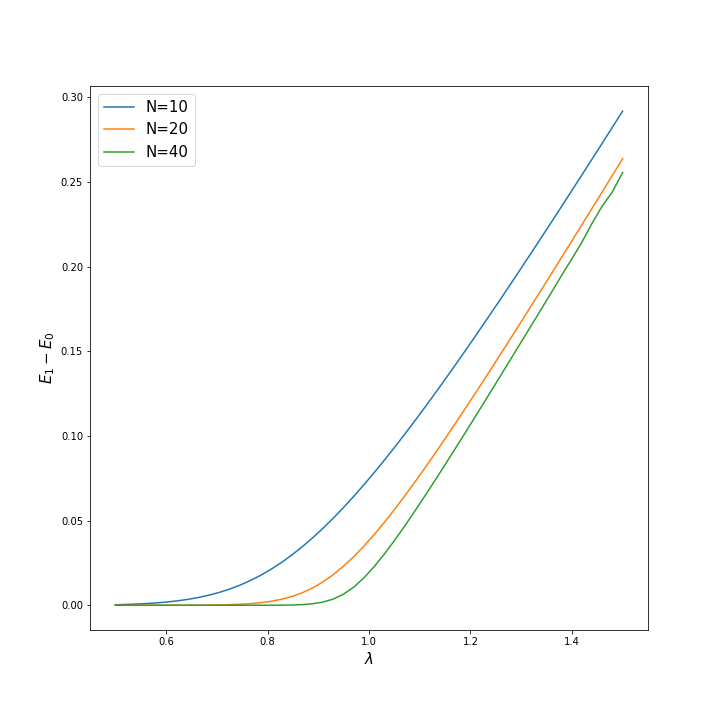
\includegraphics[width=0.7\linewidth]{graphs/energapplot}
	\caption{}
	\label{fig:energapplot}
\end{figure}


\chapter{Analitical Calculations for the XY model}
In this Chapter we will find an analytical expression for the quantities we described in chap. \ref{sec:measures} in a 1D space (chain) with an XY Hamiltonian :
\begin{equation}\label{eq:XYmodel}
	H_{X Y}=-\frac{1}{2} \sum_{l}\left(\frac{1+\gamma}{2} \sigma_{l}^{x} \sigma_{l+1}^{x}+\frac{1-\gamma}{2} \sigma_{l}^{y} \sigma_{l+1}^{y}+\lambda \sigma_{l}^{z}\right)
\end{equation}
With $\gamma, \lambda \in [0,\infty]$.\\
We will calculate the reduced density matrix on $L$ sites for the ground state of the XY model.

	To get the reduced density matrix we will follow the road map described in \cite{latorre2003ground}:
\begin{enumerate}
	\item Transform the Hamiltonian using Majorana operators
	\item Write the correlation matrix for the new operators on the ground state of the whole chain
	\item Restrict the correlation matrix to the subsystem of interest
	\item Expand the reduced density matrix in the Pauli basis
	\item Find the density matrix expectation values on the ground state using Wick's theorem 
\end{enumerate}


The non-local transformation:
\begin{equation}\label{eq:majorana}
	\check{a}_{2 l-1} \equiv\left(\prod_{m<l} \sigma_{m}^{z}\right) \sigma_{l}^{x} ; \quad
	\check{a}_{2 l} \equiv\left(\prod_{m<l} \sigma_{m}^{z}\right) \sigma_{l}^{y}
\end{equation}
\begin{equation}\label{eq:anticomm}
	\check{a}_{m}^{\dagger}=\check{a}_{m}, \quad\left\{\check{a}_{m}, \check{a}_{n}\right\}=2 \delta_{m n}\end{equation}
defines 2N Majorana operators (2 for every site: "even" and "odd") and maps the Hamiltonian \ref{eq:XYmodel} to :
\begin{equation}\label{eq:hamiltwitha}
	H =\frac{i}{2} \sum_{l=-\frac{N-1}{2}}^{\frac{N-1}{2}} \check{a}_{2 l} \check{a}_{2 l+1}  
	+ \lambda \check{a}_{2 l-1} \check{a}_{2 l}
\end{equation}
From here we can derive the correlation matrix for the Majorana operators on the ground state of the whole chain (the details of the calculation are shown in \ref{appendixcalculation}):
\begin{equation}\label{eq:corrmatr1}
	\left\langle\check{a}_{m} \check{a}_{n}\right\rangle=\delta_{m n}+i\left(\Gamma^{A}\right)_{m n}, 
\end{equation}

\begin{equation}\label{eq:corrmatr2}
	\Gamma^{A}=\left[\begin{array}{cccc}
		\Pi_{0} & \Pi_{1} & \cdots & \Pi_{N-1} \\
		-\Pi_{1}^T & \Pi_{0} & & \vdots \\
		\vdots & & \ddots & \vdots \\
		-\Pi_{N-1}^T & \cdots & \cdots & \Pi_{0}
	\end{array}\right]\end{equation}

\begin{equation}\label{eq:corrmatr3}
	\Pi_{l}=\left[\begin{array}{cc}
		0 & g_{l} \\
		-g_{-l} & 0
	\end{array}\right] 
	\quad g_{l}=\frac{1}{2 \pi} \int_{0}^{2 \pi} d \phi e^{-i l \phi} \frac{\lambda-\cos \phi+i \gamma \sin \phi}{|\lambda-\cos\phi +i  \gamma\sin \phi|}\end{equation}	 
\newline
Now if we expand the L sites density matrix in the Pauli basis:
\begin{equation}\label{eq:rhoexpansion}\rho_{L}=2^{-L} \sum_{\mu_{1}, \cdots, \mu_{L}=0, x, y, z} \rho_{\mu_{1} \cdots \mu_{L}} \sigma_{1}^{\mu_{1}} \cdots \sigma_{L}^{\mu_{L}}\end{equation}
We need only to calculate the expectation values on the ground state:
\begin{equation}\label{eq:expectation_values}
	\rho_{\mu_{1} \cdots \mu_{L}}=\left\langle\sigma_{1}^{\mu_{1}} \cdots \sigma_{L}^{\mu_{L}}\right\rangle
\end{equation}
And this can be done using: the majorana basis (\ref{eq:majorana}), Wick's theorem and the L sites-restricted correlation matrix $\Gamma^{A}_L$
\begin{equation}\label{eq:corrmatrrestrict}
	\Gamma^{A}_L=\left[\begin{array}{cccc}
		\Pi_{0} & \Pi_{1} & \cdots & \Pi_{L-1} \\
		-\Pi_{1}^T & \Pi_{0} & & \vdots \\
		\vdots & & \ddots & \vdots \\
		-\Pi_{L-1}^T & \cdots & \cdots & \Pi_{0}
	\end{array}\right]\end{equation}\\
We'll need the inverse transformations of \ref{eq:majorana}
\begin{equation}\label{eq:inversez}
	\sigma_{l}^{z} = -i\check{a}_{2l-1} \check{a}_{2 l} 
\end{equation}
\begin{equation}\label{eq:inversex}
	\sigma_{l}^{x}= \left(\prod_{m<l} \sigma_{m}^{z}\right)\check{a}_{2l-1}=
	\left(\prod_{m<l} -i\check{a}_{2m-1} \check{a}_{2 m}\right)\check{a}_{2l-1}
\end{equation}
\begin{equation}\label{eq:inversey}
	\sigma_{l}^{y}=
	\left(\prod_{m<l} -i\check{a}_{2m-1} \check{a}_{2 m}\right)\check{a}_{2l}
\end{equation}
\section{One site}

\subsection{Eigenvalues}

\begin{equation}
	\langle\check{a}_{m} \check{a}_{n}\rangle=\delta_{m n}+i\Gamma_1^A= \left[\begin{array}{cc}
		1 & 0 \\
		0 & 1
	\end{array}\right]+i\left[\begin{array}{cc}
		0 & g_0 \\
		-g_0 & 0
	\end{array}\right]
\end{equation}
$\Gamma^A_1$ is in the block diagonal form, so 
The density matrix $\rho_1$ has eigenvalues:\\
\begin{equation}\label{eq:eigonesite}
	p_1=(1+g_0)/2 \quad p_2=(1-g_0)/2
\end{equation}
\begin{equation}
	p_1=(1+	\langle{\sigma}_{1}^{z}\rangle)/2 \quad p_2=(1-	\langle{\sigma}_{1}^{z}\rangle)/2
\end{equation}\\


\subsection{Reduced Density Matrix}


We want to calculate (\ref{eq:rhoexpansion}-\ref{eq:expectation_values}):
\begin{equation}
	\rho_{1}=\frac{1}{2}\sum_{\mu_{1}=0, x, y, z} \rho_{\mu_{1}} \sigma_{1}^{\mu_{1}} 
\end{equation}
where:
\begin{equation}\label{eq:1sitepauli}
	\rho_{\mu_{1}}=\left\langle\sigma_{1}^{\mu_{1}}\right\rangle \quad \mu_{1}=0, x, y, z
\end{equation}
are the expectation values on the ground state.\\
First we express the pauli matrices in the Majorana basis using the inverse transformation of \ref{eq:majorana}:
\begin{equation}
	\sigma_1^x=\check{a}_1  \quad
	\sigma_1^y=\check{a}_2  \quad
	\sigma_1^z=-i\check{a}_1\check{a}_2
\end{equation}
And now looking at the L=1 correlation matrix  \ref{eq:corrmatrrestrict} $\Gamma^{A}_1$:
\begin{equation}
	\Gamma^{A}_1=
	\Pi_{0} = \left[\begin{array}{cc}
		0 & g_0 \\
		-g_0 & 0
	\end{array}\right]
\end{equation}\\
we are able to write all the possible expectation values of the Majorana operators (\ref{eq:corrmatr1}):
\begin{equation}
	\langle\check{a}_{m} \check{a}_{n}\rangle= \left[\begin{array}{cc}
		1 & 0 \\
		0 & 1
	\end{array}\right]+i\left[\begin{array}{cc}
		0 & g_0 \\
		-g_0 & 0
	\end{array}\right]
	\quad m,n=1,2
\end{equation}
We obtain:
\begin{equation}
	\rho_{1}=\frac{1}{2} \rho_{0} \sigma_{1}^{0} + \frac{1}{2} \rho_{z} \sigma_{1}^{z}=\frac{1}{2} \sigma_{1}^{0}+\frac{1}{2} g_0\sigma_{1}^{z}
\end{equation}
So:
\begin{equation}
	\rho_{1}=\frac{1}{2}\left[\begin{array}{cc}
		1+g_0 & 0 \\
		0 & 1-g_0
	\end{array}\right]
 =\frac{1}{2}\left[\begin{array}{cc}
		1+\langle{\sigma}_{1}^{z}\rangle & 0 \\
		0 & 1-\langle{\sigma}_{1}^{z}\rangle
	\end{array}\right]
\end{equation}
with:
\begin{equation}\label{eq:g_0coff}
	g_0=	\langle{\sigma}_{1}^{z}\rangle = \frac{1}{2 \pi} \int_{0}^{2 \pi} d \phi \frac{\lambda-\cos \phi+i \gamma\sin \phi}{|\lambda-\cos\phi +i  \gamma \sin \phi|}
\end{equation}
We plot  $(1+g_0)/2$ in fig. \ref{fig:firsteig_rho1}
\\

\subsection{Ergotropy}

\begin{equation}
	\rho_{1}=\frac{1}{2}\left[\begin{array}{cc}
		1+\langle{\sigma}_{1}^{z}\rangle & 0 \\
		0 & 1-\langle{\sigma}_{1}^{z}\rangle
	\end{array}\right]
\end{equation}

\begin{equation}
	H_1=-\frac{\lambda}{2}\sigma^z=\frac{1}{2}\left[\begin{array}{cc}
		-\lambda  & 0 \\
		0 & \lambda 
	\end{array}\right]
\end{equation}

\begin{equation}
	\mathcal{W}_1 (\rho, H)=\tr(\rho_1 H_1)-\tr(\rho_{pas 1} H_1)=0
\end{equation}
Because $\rho_1$ is already a passive state.

\subsection{Max-Ergotropy}

The density matrix $\rho_1$ has eigenvalues \ref{eq:eigonesite}:
\begin{equation}
	p_1=(1+g_0)/2 \quad p_2=(1-g_0)/2
\end{equation}\\
With $g_0 =\langle{\sigma}_{1}^{z}\rangle$  (fig. \ref{fig:g0gammas}) :

\begin{equation}\label{eq:g_0coff2}
	g_0=\frac{1}{2 \pi} \int_{0}^{2 \pi} d \phi \frac{\lambda-\cos \phi+i \gamma  \sin \phi}{|\lambda-\cos\phi +i \gamma \sin \phi|}
\end{equation}


\begin{itemize}
	\item Purity: 
	
	\begin{equation}
		\mathfrak{P}_1=\sum_{i}\left(p_{i}\right)^{2}=\frac{1+g_0^2}{2}=\frac{1+\langle{\sigma}_{1}^{z}\rangle^2}{2}
	\end{equation}
	\item Max-Ergo:
	
	\begin{equation}
		\mathcal{M}_1=2 \sum_{i=1}^{D / 2}\left(p_{i}^{(\downarrow)}-p_{D-i+1}^{(\downarrow)}\right)\left|\epsilon_{i}^{(\uparrow)}\right|=2(p_1^{(\downarrow)}-p_2^{(\downarrow)})\abs{\varepsilon_1^{(\uparrow)}}=2g_0\abs{\frac{\lambda}{2}}=g_0\abs{\lambda}=\langle{\sigma}_{1}^{z}\rangle\abs{\lambda}
	\end{equation}
	\item Rescaled-Max-Ergotropy
	\begin{equation}
		\mathfrak{M}_1=g_0=\langle{\sigma}_{1}^{z}\rangle
	\end{equation}	
	
\end{itemize}
The second derivative with respect to $\lambda$ of the Max-Ergotropy is very sensible to the phase transition (fig. \ref{fig:onesitesecdev})

\clearpage
\subsection{Graphs}

\begin{figure}[h]
	\centering
	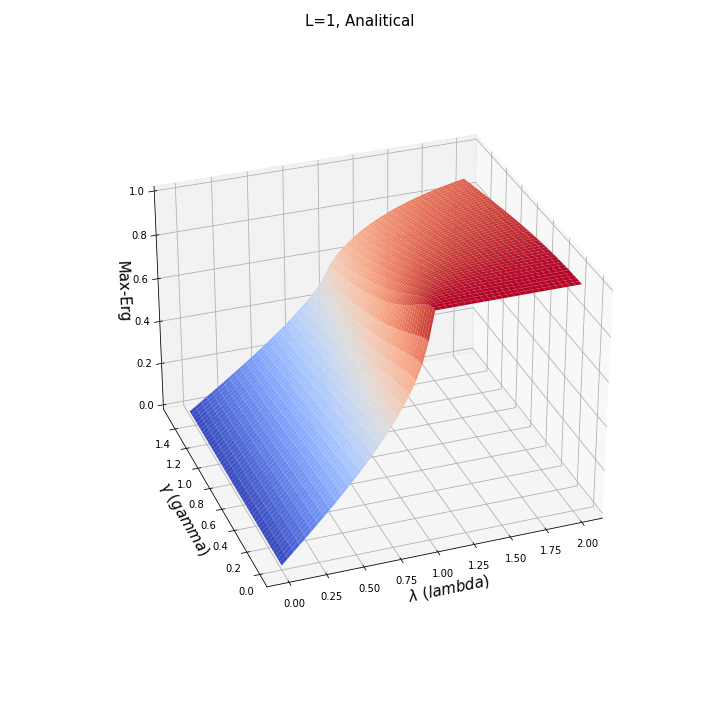
\includegraphics[width=\linewidth]{graphs/3dplot_g0}
	\caption{For One Site, the Max-Ergotropy corresponds to the $g_0 = \langle{\sigma}_{1}^{z}\rangle$ coefficient.   }
	\label{fig:g0gammas}
\end{figure}
\begin{figure}[h]
	\centering
	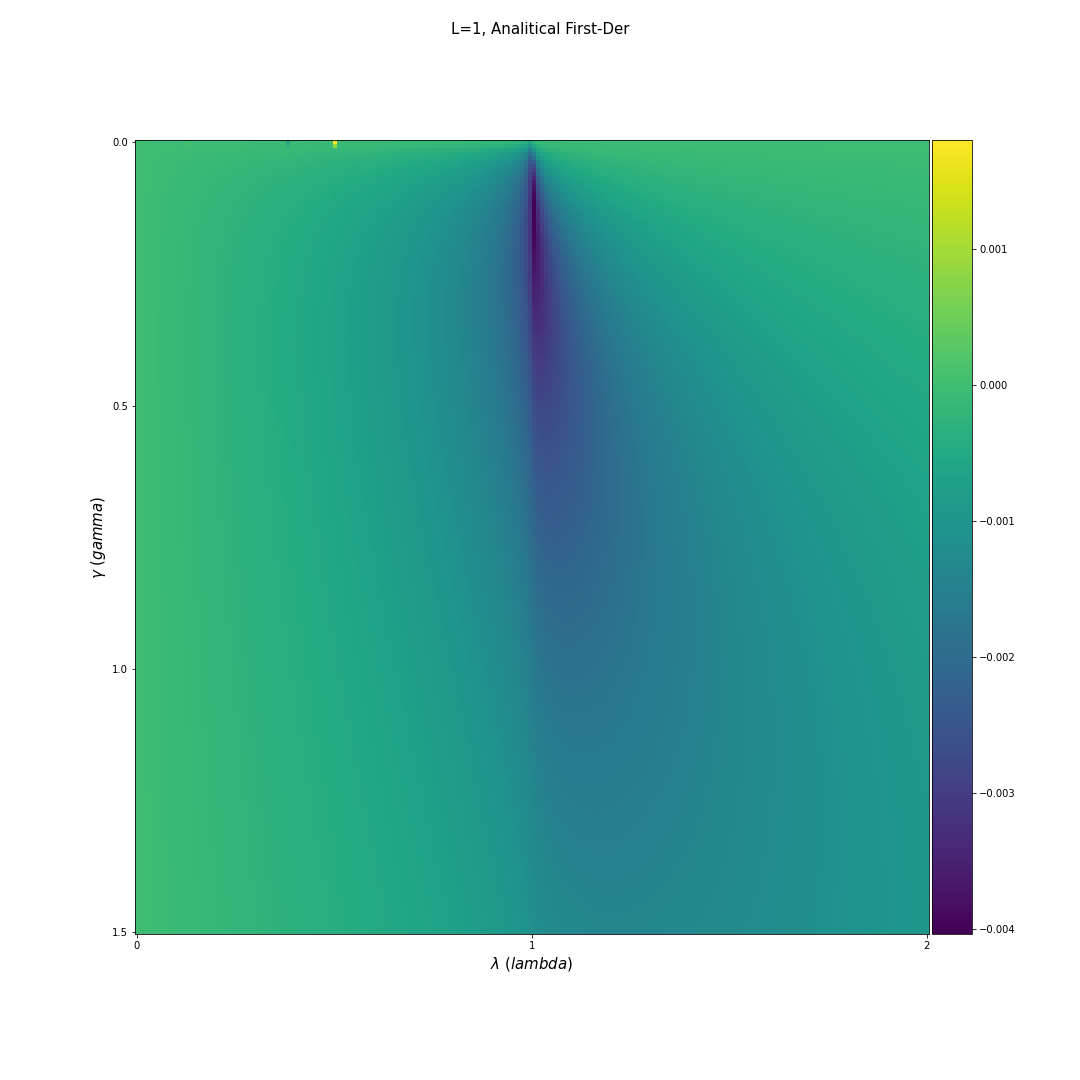
\includegraphics[width=\linewidth]{./graphs/planarplot_firstder_onesite}
	\caption{First-Derivative one-site Max-Ergotropy ($g_0$)}
	\label{fig:onesitesecdev}
\end{figure}

\clearpage
\section{Two sites}

\subsection{Eigenvalues}
Eigenvalues of the correlation matrix
\begin{equation}
	\nu_{\pm}=\sqrt{\left(\frac{g_{1}-g_{-1}}{2}\right)^{2}+g_{0}^{2}} \pm \left| \frac{g_{1}+g_{-1}}{2} \right|
\end{equation}
With $\nu_-<\nu_+$.\\
These eigenvalues can be interpreted as occupation numbers for the fermionic modes  \cite{Franchini_2014} \cite{latorre2003ground}:

\begin{equation}
	\left\langle\hat{c}_{m} \hat{c}_{n}\right\rangle=0, \quad\left\langle\hat{c}_{m}^{\dagger} \hat{c}_{n}\right\rangle=\delta_{m n} \frac{1+\nu_{m}}{2} \quad m,n=+,-
\end{equation}
Where the $\hat{c}$ operators are particular combinations of the Majorana operators that diagonalize the correlation matrix.\\
Eigenvalues of the density matrix:

\begin{equation}
	p_{\pm \pm } =(1 \pm \nu_-)(1 \pm \nu_+)/4
\end{equation}

\subsection{Reduced Density Matrix}
	We want to calculate the density matrix for 2 adjacent sites in the infinite XY chain.\\ We'll need the expectations values on the ground state for:
\begin{equation}\label{eq:2sitepauli}
	\rho_{\mu_{1}  \mu_{2}}=\left\langle\sigma_{1}^{\mu_{1}}  \sigma_{2}^{\mu_{2}}\right\rangle \quad \mu_{1},\mu_{2}=0, x, y, z
\end{equation}
Using the inverse transformations of \ref{eq:majorana} :

\begin{equation}
	\sigma_1^z=-i\check{a}_1\check{a}_2 \quad
	\sigma_2^z=-i\check{a}_3\check{a}_4
\end{equation}
\begin{equation}
	\sigma_1^x=\check{a}_1 \quad \sigma_2^x=-i\check{a}_1\check{a}_2\check{a}_3
\end{equation}
\begin{equation}
	\sigma_1^y=\check{a}_2 \quad \sigma_2^y=-i\check{a}_1\check{a}_2\check{a}_4
\end{equation}
The correlation matrix for the first 4 Majorana operators is ( \ref{eq:corrmatr3} , \ref{eq:corrmatrrestrict} ):
\begin{equation}\label{eq:corrmatr2sites1}
	\left\langle\check{a}_{m} \check{a}_{n}\right\rangle=\delta_{m n}+i\left(\Gamma_{2}^{A}\right)_{m n}, \quad m, n=1,2,3,4
\end{equation}
\begin{equation}\label{eq:corrmatr2sites2}
	\Gamma_{2}^{A}=\left[\begin{array}{cc}
		\Pi_0 & \Pi_1 \\
		-\Pi_1^T & \Pi_0
	\end{array}\right]
	=\left[\begin{array}{cccc}
		0 & g_0 & 0& g_1\\
		-g_0 & 0 &-g_{-1} & 0\\
		0&g_{-1}&0&g_0\\
		-g_1&0&-g_0& 0
	\end{array}\right]
\end{equation}

\begin{equation}
	g_l=\frac{1}{2 \pi} \int_{0}^{2 \pi} d \phi e^{-i l \phi} \frac{\lambda-\cos \phi+i \gamma \sin \phi}{|\lambda-\cos\phi +i  \gamma \sin \phi|}
\end{equation}

Now we have all we need to calculate  the coefficients of the 2-site density matrix in the pauli basis on the ground state ( \ref{eq:2sitepauli} ) using Wick's theorem.\\
The Hamiltonian \ref{eq:XYmodel} has a symmetry:
\begin{equation}\label{eq:symm}\left(\prod_{l} \sigma_{l}^{z}\right) H\left(\prod_{l} \sigma_{l}^{z}\right)=H\end{equation}
That allows us to say that:
\begin{equation}\rho_{\mu_{1}\cdots  \mu_{L}}=\left\langle\sigma_{1}^{\mu_{1}}\cdots  \sigma_{L}^{\mu_{L}}\right\rangle=0 \quad \text{if the sum of $\mu=x$ and $\mu=y$ is odd}\end{equation}
For example in our case ($L=2$): $\rho_{x0}=\rho_{zy}=0$ \\
The only non-vanishing terms are:
\begin{equation}
	\rho_{00}\quad \rho_{xx} \quad \rho_{yy} \quad \rho_{xy} \quad \rho_{yx} \quad \rho_{zz}
	\quad \rho_{z0} \quad \rho_{0z}
\end{equation}
We now use Wick's theorem:
\begin{equation}\label{eq:wickcalc}
	\begin{aligned}
		&\rho_{xx}=\left\langle\sigma_{1}^{x} \sigma_{2}^{x}\right\rangle=
		-i\left\langle\check{a}_1\check{a}_1\check{a}_2\check{a}_3\right\rangle \\ &=-i\left\langle\check{a}_1\check{a}_1\right\rangle\left\langle\check{a}_2\check{a}_3\right\rangle+ i\left\langle\check{a}_1\check{a}_2\right\rangle\left\langle\check{a}_1\check{a}_3\right\rangle
		-i\left\langle\check{a}_1\check{a}_3\right\rangle\left\langle\check{a}_1\check{a}_2\right\rangle=-i(-ig_{-1})+0-0 \\ 		
		&\rho_{yy}=-i\left\langle\check{a}_2\check{a}_1\check{a}_2\check{a}_4\right\rangle=\\&=-i\left\langle\check{a}_2\check{a}_1\right\rangle\left\langle\check{a}_2\check{a}_4\right\rangle+i\left\langle\check{a}_2\check{a}_2\right\rangle\left\langle\check{a}_1\check{a}_4\right\rangle-i\left\langle\check{a}_2\check{a}_4\right\rangle\left\langle\check{a}_1\check{a}_2\right\rangle=0+i(ig_1)-0 \\ 	
		&\rho_{xy}=-i\left\langle\check{a}_1\check{a}_1\check{a}_2\check{a}_4\right\rangle=\\&=-i\left\langle\check{a}_1\check{a}_1\right\rangle\left\langle\check{a}_2\check{a}_4\right\rangle+i\left\langle\check{a}_1\check{a}_2\right\rangle\left\langle\check{a}_1\check{a}_4\right\rangle-i\left\langle\check{a}_1\check{a}_4\right\rangle\left\langle\check{a}_1\check{a}_2\right\rangle=0+i(ig_0ig_1)-i(ig_1ig_0) \\ 
		&\rho_{yx}=-i\left\langle\check{a}_2\check{a}_1\check{a}_2\check{a}_3\right\rangle=\\&=-i\left\langle\check{a}_2\check{a}_1\right\rangle\left\langle\check{a}_2\check{a}_3\right\rangle+ i\left\langle\check{a}_2\check{a}_2\right\rangle\left\langle\check{a}_1\check{a}_3\right\rangle
		-i\left\langle\check{a}_2\check{a}_3\right\rangle\left\langle\check{a}_1\check{a}_2\right\rangle=ig_0g_{-1}+0-ig_0g_{-1} \\ 
		&\rho_{zz}=-\left\langle\check{a}_1\check{a}_2\check{a}_3\check{a}_4\right\rangle=\\&=-\left\langle\check{a}_1\check{a}_2\right\rangle\left\langle\check{a}_3\check{a}_4\right\rangle+\left\langle\check{a}_1\check{a}_3\right\rangle\left\langle\check{a}_2\check{a}_4\right\rangle-\left\langle\check{a}_1\check{a}_4\right\rangle\left\langle\check{a}_2\check{a}_3\right\rangle=-ig_0ig_{0}+0-(ig_1(-ig_{-1})) \\ 
		&\rho_{z0}=-i\left\langle\check{a}_1\check{a}_2\right\rangle=-i(ig_0) \quad  \rho_{0z}=-i\left\langle\check{a}_3\check{a}_4\right\rangle=-i(ig_{0})	 \quad		\rho_{00}=1 \\
	\end{aligned}	
\end{equation}
So:
\begin{equation}\label{eq:coeff2sites}
	\begin{gathered}
		\rho_{00}=1 \qquad
		\rho_{xx}=-g_{-1} \qquad \rho_{yy}=-g_1 \qquad \rho_{xy}=0  \\
		\\ \rho_{yx}=0 \qquad
		\rho_{zz}=g_{0}^2-g_1g_{-1} \qquad \rho_{z0}=\rho_{0z}=g_0 \\
	\end{gathered}
\end{equation}
Using \ref{eq:rhoexpansion}:
\begin{equation}
	\rho_2=\frac{1}{4} [ ( \sigma_1^0 \otimes\sigma_2^0 ) -g_{-1} \left(\sigma_1^x \otimes\sigma_2^x\right) - g_{1} \left(\sigma_1^y \otimes\sigma_2^y\right) + (g_{0}^2-g_1g_{-1}) \left(\sigma_1^z \otimes\sigma_2^z\right)+g_0\left(\sigma_1^0 \otimes\sigma_2^z+\sigma_1^z \otimes\sigma_2^0\right) ] 
 \end{equation}

\newpage
\subsection{Ergotropy}
\begin{equation}
	\rho_2=\frac{1}{4}  [ ( \sigma_1^0 \sigma_2^0 ) -g_{-1} \left(\sigma_1^x \sigma_2^x\right) - g_{1} \left(\sigma_1^y \sigma_2^y\right) + (g_{0}^2-g_1g_{-1}) \left(\sigma_1^z \sigma_2^z\right)+g_0\left(\sigma_1^0 \sigma_2^z+\sigma_1^z \sigma_2^0\right) ] 
\end{equation}
\begin{equation}\label{eq:rho2explicit}
	\frac{1}{4}\mathbb{Id} + \frac{1}{4} \left[
	\begin{array}{cccc}
		g_0^2+2g_0-g_{-1} g_1&  &  & g_1-g_{-1} \\
		& g_{-1} g_1-g_0^2 &-g_1-g_{-1}  &  \\
		& -g_1-g_{-1} & g_{-1} g_1-g_0^2 &  \\
		g_1-g_{-1}&  &  &  g_0^2-2g_0-g_{-1} g_1
	\end{array}\right]
\end{equation}
For $\lambda \rightarrow \infty $ : $g_l =\delta_{0,l}$ \\







For the Ising Model ($\gamma=1$) , $g_1=0$ at $\lambda=0$, so that:
\begin{equation} 
	\rho_2=	\frac{1}{4} \left( \sigma_1^0 \sigma_2^0 + \sigma_1^x \sigma_2^x \right)
\end{equation}
as we expect.\\

The eigenvalues of \ref{eq:rho2explicit} are:
(first two middle ones)
\begin{equation}
	\begin{aligned} &
		\frac{1}{4}
		\left\{ \left(1-g_0^2+g_{-1} g_1 -g_{-1}-g_1\right), \left(1-g_0^2+g_{-1} g_1+g_{-1}+g_1\right), \right. \\
		&\left. \left(1+g_0^2-g_{-1} g_1-\sqrt{4 g_0^2+(g_1-g_{-1})^2}\right),
		\left(1+g_0^2-g_{-1} g_1+\sqrt{4 g_0^2+(g_1-g_{-1})^2}\right)\right\}
	\end{aligned}
\end{equation}
\begin{equation}
	\begin{aligned} 
		&\frac{1}{4}
		\left\{(1+\nu_-)(1-\nu_+), (1-\nu_-)(1+\nu_+) \right. \\
		&\left. (1-\nu_-)(1-\nu_+),
		(1+\nu_-)(1+\nu_+)\right\}
	\end{aligned}
\end{equation}
\begin{figure}[h]
	\centering
	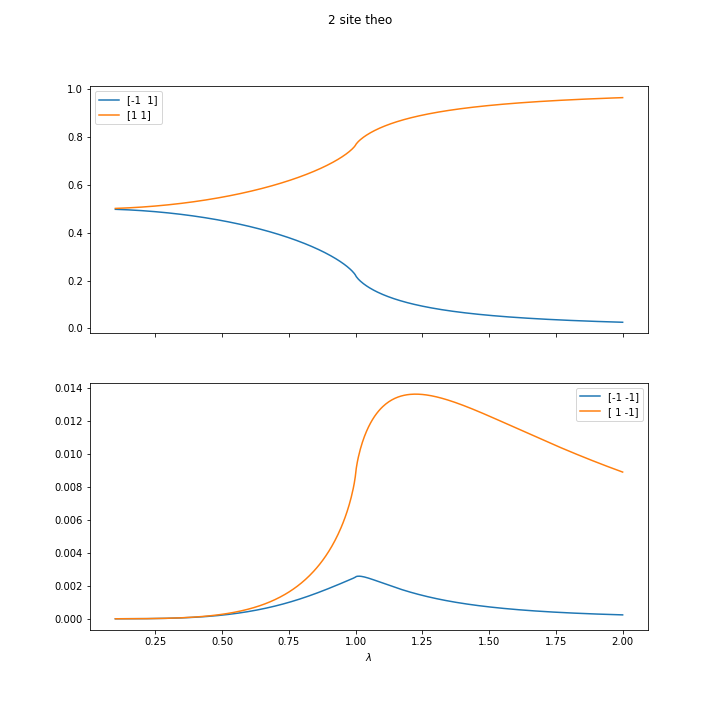
\includegraphics[width=0.7\linewidth]{graphs/two_site_theo}
	\caption{Eigenvalues of the two-site density matrix}
	\label{fig:twositetheo}
\end{figure}
If we want to sort them, it's easy for $\gamma>1$: (for $\gamma<1$ there's a problem  at low lambdas but we can solve it focusing only on the region $\lambda \simeq 1 $) \\
Descending (up to down) order of the eigenvalues of the rdm: fig.\ref{fig:twositetheo}
\begin{equation}
\begin{array}{c}
	1/4(1+\nu_-)(1+\nu_+)\\ 
	1/4(1-\nu_-)(1+\nu_+)\\
	1/4(1+\nu_-)(1-\nu_+)\\
	1/4(1-\nu_-)(1-\nu_+) \\ 
\end{array}
\end{equation}
For now we consider $\lambda \simeq 1$ or we have troubles with ordering\\
Eigenvalues of 2 site Hamiltonian in ascending order:
\begin{equation}
\left\{-\frac{1}{2} \sqrt{\gamma ^2+4 \lambda ^2},-\frac{1}{2},\frac{1}{2},\frac{1}{2} \sqrt{\gamma ^2+4 \lambda ^2}\right\}
\end{equation}

for $\gamma=1$:
\begin{equation}
	\left\{-\frac{1}{2} \sqrt{1+4 \lambda ^2},-\frac{1}{2},\frac{1}{2},\frac{1}{2} \sqrt{1+4 \lambda ^2}\right\}
\end{equation}

Ergotropy:
\begin{equation}
	\mathcal{W}(\rho,H)=E(\rho)-E(\rho_{pas})=\sum_{j, k} r_{j}^{(\downarrow)} \varepsilon_{k}^{(\uparrow)}\left( \left|\braket{r_j^{(\downarrow)}}{\varepsilon_{k}^{(\uparrow)}}\right|^2-\delta_{jk}\right)
\end{equation} 

\begin{equation}
E(\rho_{pas})=
\left[ \begin{array}{c}
	1/4(1+\nu_-)(1+\nu_+)\\ 
	1/4(1-\nu_-)(1+\nu_+)\\
	1/4(1+\nu_-)(1-\nu_+)\\
	1/4(1-\nu_-)(1-\nu_+) \\ 
\end{array} \right]
\left[
\begin{array}{cccc}
	-\frac{1}{2}\sqrt{\gamma ^2+4 \lambda ^2}	& -\frac{1}{2} & \frac{1}{2} & \frac{1}{2} \sqrt{\gamma ^2+4 \lambda ^2} \\
\end{array} \right]
\end{equation}

\begin{equation}
	E(\rho_{pas})=
	-\frac{1}{4} \left(\sqrt{(g_{-1}- g_1)^2 +4 g_0^2} \left(\sqrt{\gamma ^2+4 \lambda ^2}\right)-g_{-1}-g_1\right)
\end{equation}
\begin{equation}
	E(\rho_{pas})=
	-\frac{1}{4} \left(( \nu_+ + \nu_-) \left(\sqrt{\gamma ^2+4 \lambda ^2}\right)+(\nu_+ - \nu_-)\right)
\end{equation}
\begin{equation}
E(\rho)=\frac{1}{4} \left((\gamma +1) g_{-1}-(\gamma -1) g_1-4 g_0 \lambda \right)
\end{equation}
$\gamma=1$:
\begin{equation}
E(\rho)= 1/2(g_{-1}-2\lambda g_0)
\end{equation}

Due to symmetry in H: $E(\rho_{pass})$ is -$E(\rho_{antipass})$ \\
Ergotropy:
\begin{equation}
	\frac{1}{4} \left(\sqrt{(g_{-1}- g_1)^2+4 g_0^2} \sqrt{\gamma ^2+4 \lambda ^2}+\gamma  g_{-1}-\gamma  g_1-4 g_0 \lambda \right)
\end{equation}
for $\gamma=1$ :\\
\begin{equation}
\frac{1}{4} \left(\sqrt{(g_{-1}- g_1)^2 +4 g_0^2} \left(\sqrt{4 \lambda ^2+1}\right)+ g_{-1}-4 g_0 \lambda -g_1\right)
\end{equation}


\clearpage
\subsection{Max-Ergotropy}\label{sec:max_twosites}


Eigenvalues of the density matrix:

\begin{equation}
	p_{\pm \pm } =(1 \pm \nu_-)(1 \pm \nu_+)/4
\end{equation}

Eigenvalues of 2 site Hamiltonian:
\begin{equation}
	H=-\frac{1}{2} \left(\sigma^{x} \sigma^{x}+\lambda\sigma^{z} \sigma^0+\lambda\sigma^0\sigma^{z}\right) =
	\left(
	\begin{array}{cccc}
		-\lambda  & 0 & 0 & -\frac{1}{2} \\
		0 & 0 & -\frac{1}{2} & 0 \\
		0 & -\frac{1}{2} & 0 & 0 \\
		-\frac{1}{2} & 0 & 0 & \lambda  \\
	\end{array}
	\right)
\end{equation}
\begin{equation}
	\left\{-\frac{1}{2} \sqrt{1+4 \lambda ^2},-\frac{1}{2},\frac{1}{2},,\frac{1}{2} \sqrt{1+4 \lambda ^2}\right\}
\end{equation}

\begin{equation}
	\begin{aligned}
		&
		\mathcal{M}(\mathcal{I})=2 \sum_{i=1}^ {2}\left(p_{i}^{(\downarrow)}-p_{D-i+1}^{(\downarrow)}\right)\left|\epsilon_{i}^{(\uparrow)}\right|	\\
		& \left(p_{1}^{(\downarrow)}-p_{4}^{(\downarrow)}\right)\left|\epsilon_{1}^{(\uparrow)}\right|+\left(p_{2}^{(\downarrow)}-p_{3}^{(\downarrow)}\right)\left|\epsilon_{2}^{(\uparrow)}\right|=\\
		& (1/4)\left[(1+\nu_-)(1+\nu_+)-(1-\nu_-)(1-\nu_+)\right] \left(\sqrt{1+4 \lambda ^2}\right) + \\
		&(1/4)\left[(1-\nu_-)(1+\nu_+)-(1+\nu_-)(1-\nu_+)\right] = \\
		&\frac{(\nu_+ + \nu_-)}{2}\left(\sqrt{1+4 \lambda ^2}\right)+\frac{\nu_+-\nu_-}{2} \\
	\end{aligned}
\end{equation}
Normalized:
\begin{equation}
	\mathfrak{M}(\mathcal{I}) = \frac{\mathcal{M}(\mathcal{I})}{2\left|\epsilon_{1}^{(\uparrow)}\right|} =\frac{(\nu_+ + \nu_-)}{2}+\frac{(\nu_+-\nu_-)} {2\left(\sqrt{1+4 \lambda ^2}\right)}
\end{equation}

\subsection{Graphs}



\begin{figure}[h]
	\centering
	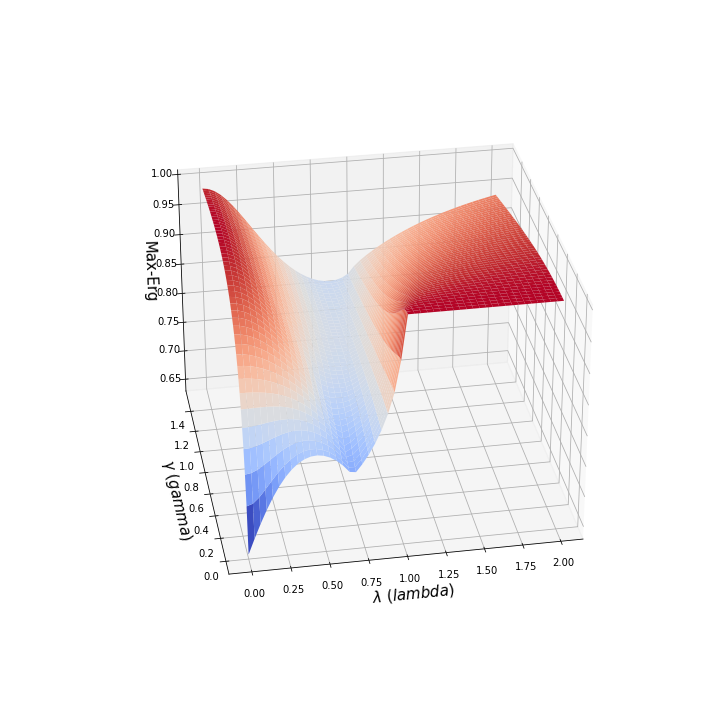
\includegraphics[width=0.7\linewidth]{graphs/3dplotmaxerg}
	\caption{Max-Ergotropy}
	\label{fig:3dplotmaxerg}
\end{figure}
\begin{figure}[h]
	\centering
	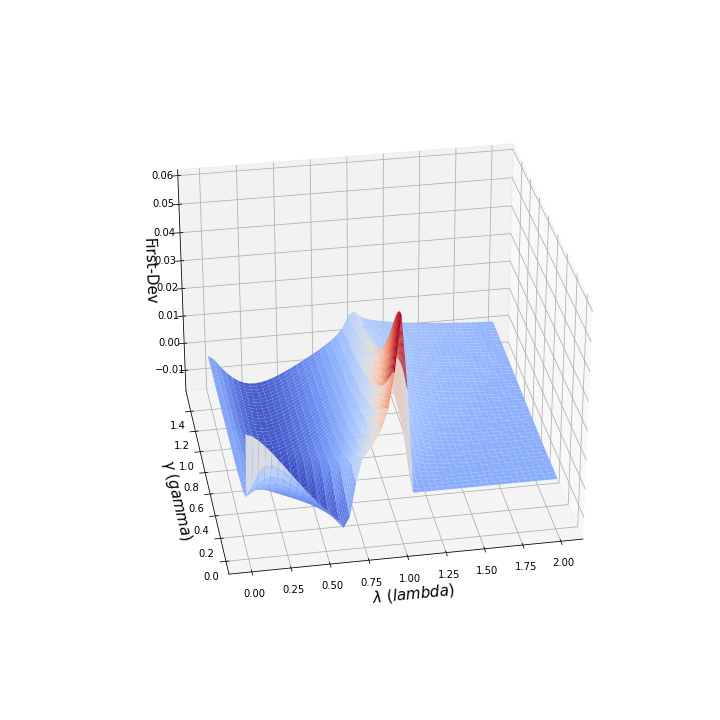
\includegraphics[width=0.7\linewidth]{graphs/3dplotfirstdevmaxerg}
	\caption{First-Derivative of the Max-Ergotropy}
	\label{fig:3dplotfirstdevmaxerg}
\end{figure}


\begin{figure}[h]
	\centering
	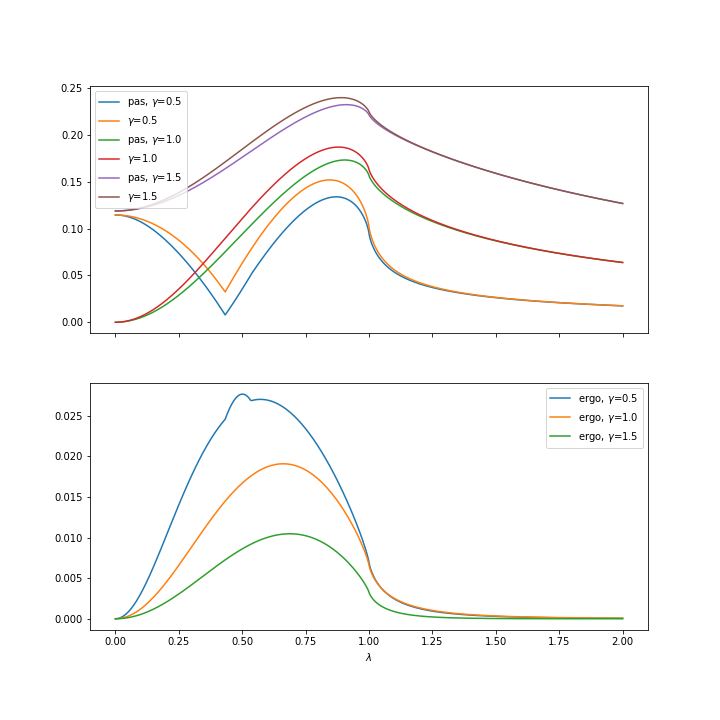
\includegraphics[width=0.7\linewidth]{graphs/Ergotheo_2sites}
	\caption{Ergotropy analitical calculation}
	\label{fig:ergotheo2sites}
\end{figure}

\clearpage
\section{Two distant sites}

\subsection{Eigenvalues}
We have to change $g_1$ with $g_d$ where d is the distance between sites. \cite{PhysRevA.78.052302}
\begin{equation}
	\nu_{\pm}=\sqrt{\left(\frac{g_{d}-g_{-d}}{2}\right)^{2}+g_{0}^{2}} \pm \left| \frac{g_{d}+g_{-d}}{2} \right|
\end{equation}
Eigenvalues of the density matrix:
\begin{equation}
	p_{\pm \pm } =(1 \pm \nu_-)(1 \pm \nu_+)/4
\end{equation}

\subsection{Reduced Density Matrix (difficult)}
If we choose two distant sites at a distance $d$:

\begin{equation}\label{eq:2distantsitespauli}
	\rho_{\mu_{1}  \mu_{2}}=\left\langle\sigma_{1}^{\mu_{1}}  \sigma_{2}^{0} \dots \sigma_{d}^{\mu_{d}}\right\rangle=\left\langle\sigma_{1}^{\mu_{1}}  \sigma_{d}^{\mu_{d}}\right\rangle \quad \mu_{1},\mu_{d}=0, x, y, z
\end{equation}

\begin{equation}
	\sigma_1^x=\check{a}_1  \quad
	\sigma_1^y=\check{a}_2  \quad
	\sigma_1^z=-i\check{a}_1\check{a}_2
\end{equation}
\begin{equation}
	\sigma_{d}^{z} = -i\check{a}_{2d-1} \check{a}_{2 d} 
\end{equation}
\begin{equation}
	\sigma_{d}^{x}=
	\left(\prod_{m<d} -i\check{a}_{2m-1} \check{a}_{2 m}\right)\check{a}_{2d-1}
\end{equation}
\begin{equation}
	\sigma_{d}^{y}=
	\left(\prod_{m<d} -i\check{a}_{2m-1} \check{a}_{2 m}\right)\check{a}_{2d}
\end{equation}
\subsection{Max-Ergotropy}

Eigenvalues of the density matrix:
\begin{equation}
	p_{\pm \pm } =(1 \pm \nu_-)(1 \pm \nu_+)/4
\end{equation}
Eigenvalues of distant Hamiltonian:
\begin{equation}
	H_{dist}=-(\lambda/2)(\sigma^z_l\sigma^0_{l+d} +\sigma^0_l\sigma^z_{l+d})
\end{equation}
\begin{equation}
	\text{eigs}= \{-\lambda,0,0 ,\lambda \}
\end{equation}
Normalized-Max-Ergo: (the two eigenvalues of the Hamiltonian are the same, so we simplify)
\begin{equation}
	\mathfrak{M}(\mathcal{I}) =	  \sum_{i=1}^ {2}\left(p_{i}^{(\downarrow)}-p_{D-i+1}^{(\downarrow)}\right) =	\frac{(\nu_+ + \nu_-)}{2}+\frac{(\nu_+-\nu_-)} {2}
\end{equation}

\clearpage

\section{More than two sites }
We stress again \cite{Latorre_2009} that  the eigenvalues of the reduced density matrix can be calculated directly from the correlation matrix in the Majorana basis (\ref{eq:corrmatr2}) because the basis  coefficients stay the same after the Jordan Wigner Trasformation:
\begin{equation}
	\begin{aligned}
		|\psi\rangle &=\sum_{i_{1}, i_{2}, \ldots, i_{n}} C^{i_{1}, i_{2}, \ldots, i_{n}}\left|i_{1}, i_{2}, \ldots, i_{n}\right\rangle \\
		&=\sum_{i_{1}, i_{2}, \ldots, i_{n}} C^{i_{1}, i_{2}, \ldots, i_{n}} (a_{1}^{\dagger})^{i_{1}}(a_{2}^{\dagger})^{i_{2}} \ldots(a_{n}^{\dagger})^{i_{n}}|\mathrm{vac}\rangle
	\end{aligned}
\end{equation}
where the $i$'s represent a spin basis and the $a$'s are the fermionic creation operators\\
So using the correlation matrix for the Majorana fermions on the ground state (\ref{eq:corrmatr1}, \ref{eq:corrmatr2}):
\begin{equation}
	\left\langle\check{a}_{m} \check{a}_{n}\right\rangle=\delta_{m n}+i\left(\Gamma^{A}\right)_{m n}, 
\end{equation}
\begin{equation}
	\Gamma^{A}=\left[\begin{array}{cccc}
		\Pi_{0} & \Pi_{1} & \cdots & \Pi_{N-1} \\
		-\Pi_{1}^T & \Pi_{0} & & \vdots \\
		\vdots & & \ddots & \vdots \\
		-\Pi_{N-1}^T & \cdots & \cdots & \Pi_{0}
	\end{array}\right]
\end{equation}
We can calculate the eigenvalues of the reduced density matrix for any group of sites we want. Basically if we want the eigenvalues for the density matrix of $L$ adiacent sites we have to:\\
 \begin{enumerate}
 	\item diagonalize the appropriate $\Gamma^A_L$ matrix
 	\item The diagonal matrix we obtain as the form: \begin{equation}
 		\Gamma_{L}^{C}=\bigoplus_{l=1}^{L}\left[\begin{array}{cc}
 			0 & \nu_{l} \\
 			-\nu_{l} & 0
 		\end{array}\right]
 	\end{equation}
So, writing:
 	\begin{equation}
 		\rho_{L}=\varrho_{1} \otimes \cdots \otimes \varrho_{L}
 	\end{equation}
The density matrix $\rho_l$ has eigenvalues:
 \begin{equation}
 	p_{l\pm}=\frac{1 \pm \nu_{l}}{2}
 \end{equation}
\item The eigenvalues of $\rho_L$ are obtained computing all the possible $p_l$ products
\end{enumerate}

\subsection{Graphs}
\begin{figure}[h]
	\centering
	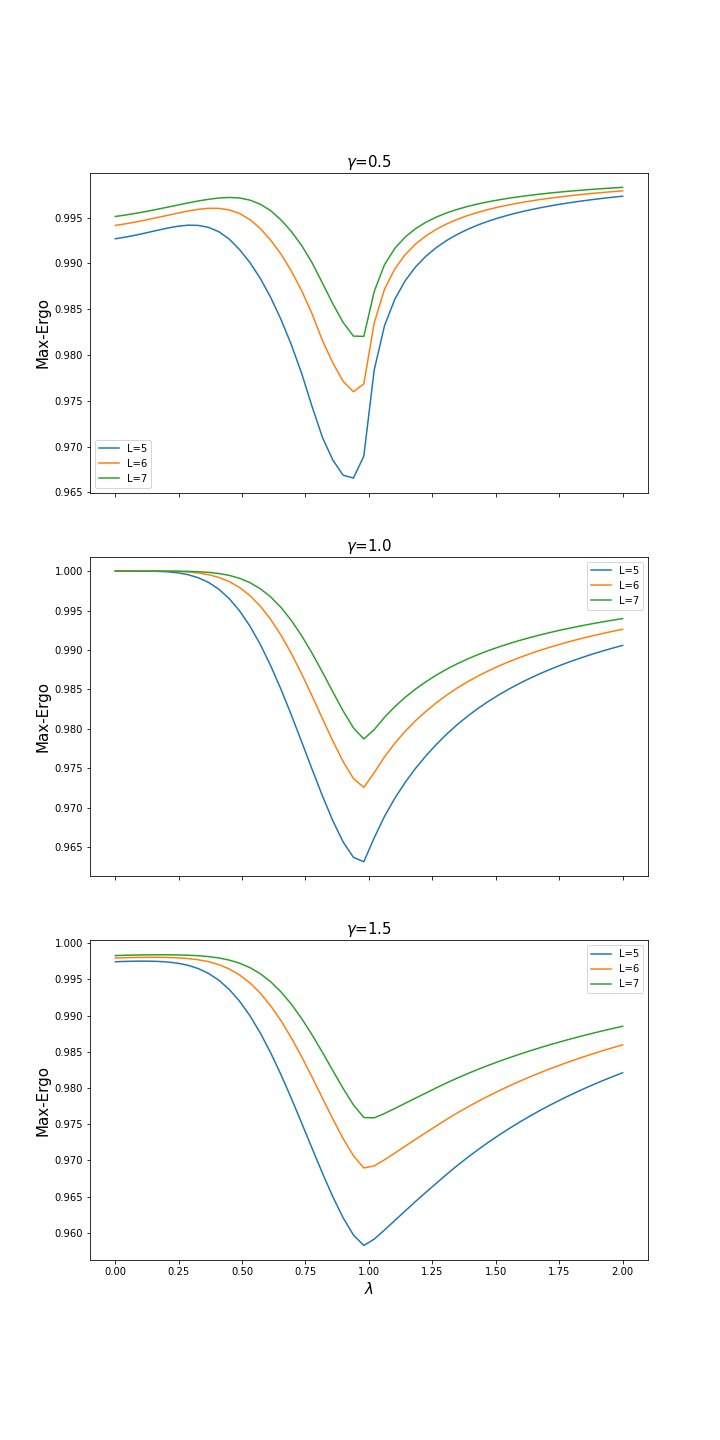
\includegraphics[width=0.7\linewidth]{graphs/Maxerg_567_3gammas}
	\caption{Analitical Max-Ergotropy}
	\label{fig:maxerg5673gammas}
\end{figure}
\begin{figure}[h]
	\centering
	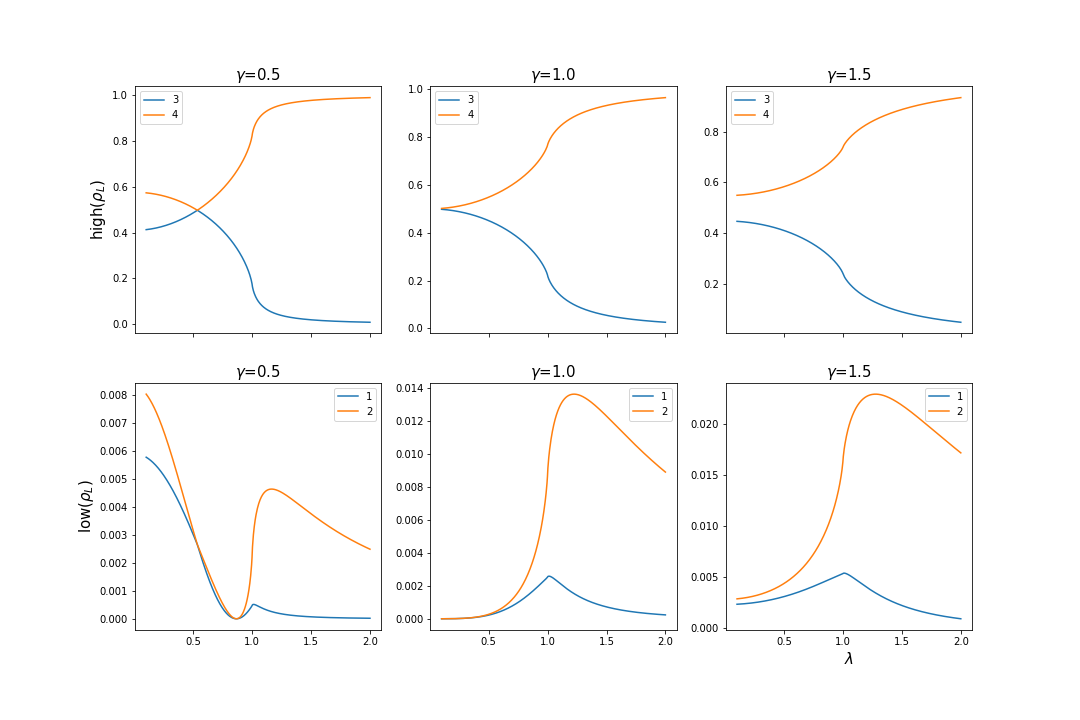
\includegraphics[width=\linewidth]{graphs/2sites_3gammas}
	\caption{Eigenvalues of the 2-sites density matrix}
	\label{fig:2sites3gammas}
\end{figure}

\begin{figure}[h]
	\centering
	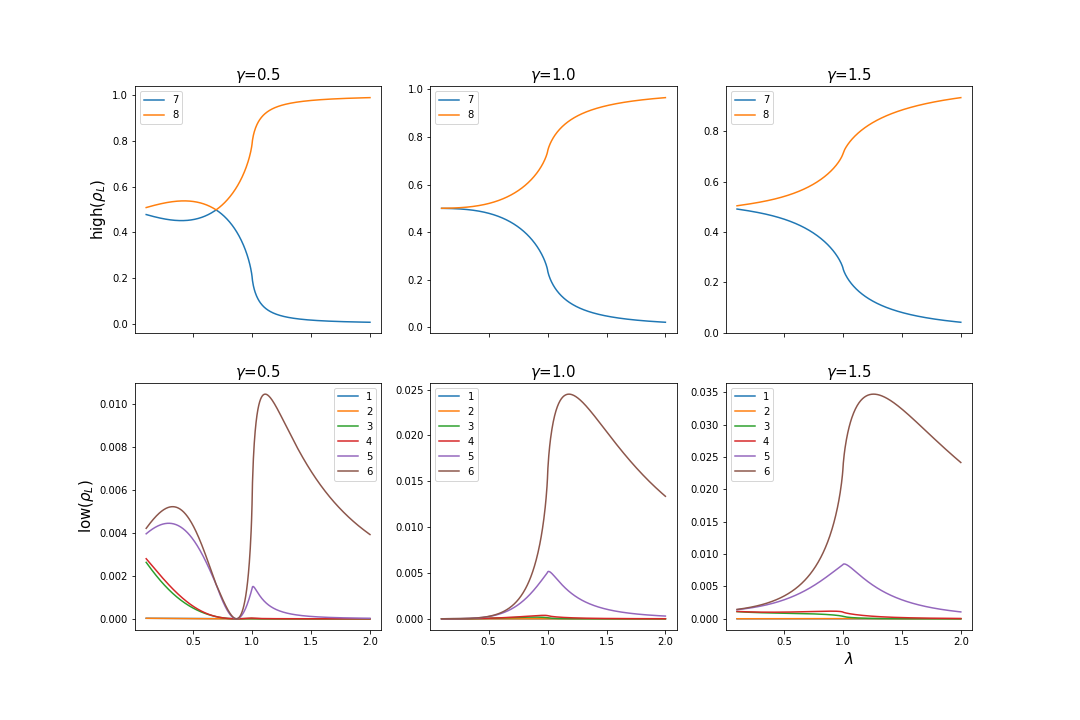
\includegraphics[width=\linewidth]{graphs/3sites_3gammas}
	\caption{Eigenvalues of the 3-sites density matrix}
	\label{fig:3sites3gammas}
\end{figure}

\begin{figure}[h]
	\centering
	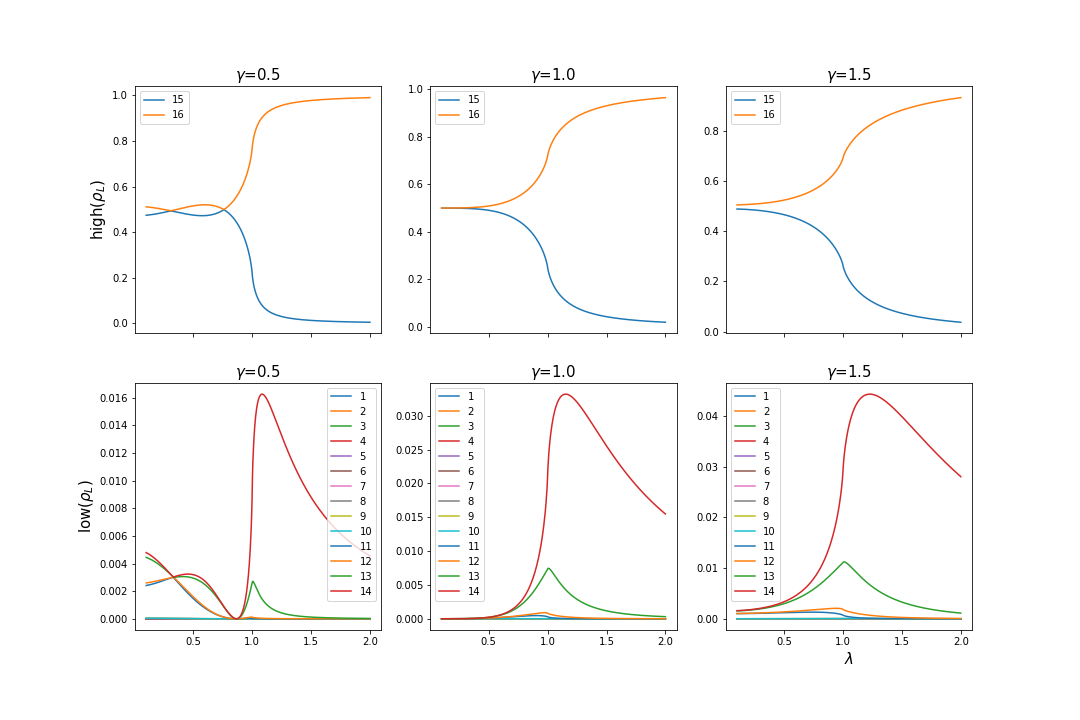
\includegraphics[width=\linewidth]{graphs/4sites_3gammas}
	\caption{Eigenvalues of the 4-sites density matrix}
	\label{fig:4sites3gammas}
\end{figure}
It's clear that only the first 2-3 eigenvalues are relevant. \\
I suppose we can stick with two sites density matrix for simulations.\\



\begin{figure}
		\centering
		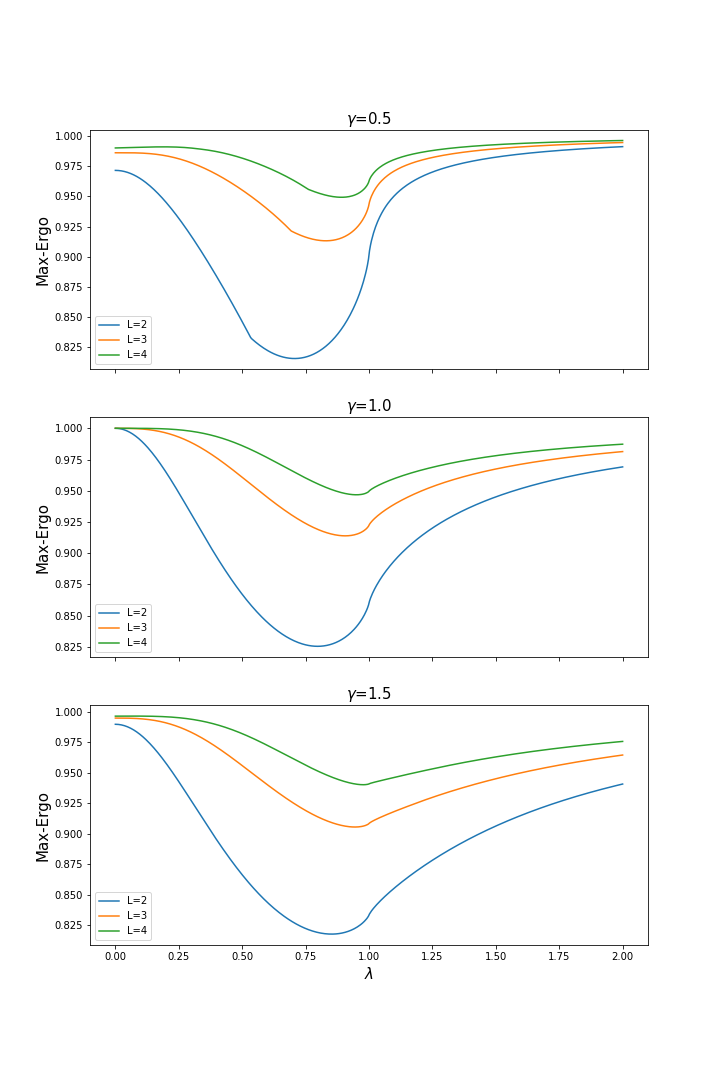
\includegraphics[width=\linewidth]{graphs/Maxerg_234_3gammas}
		\caption{Max-Ergotropy analitical calculations}
		\label{fig:maxerg2343gammas}
\end{figure}

\begin{figure}
	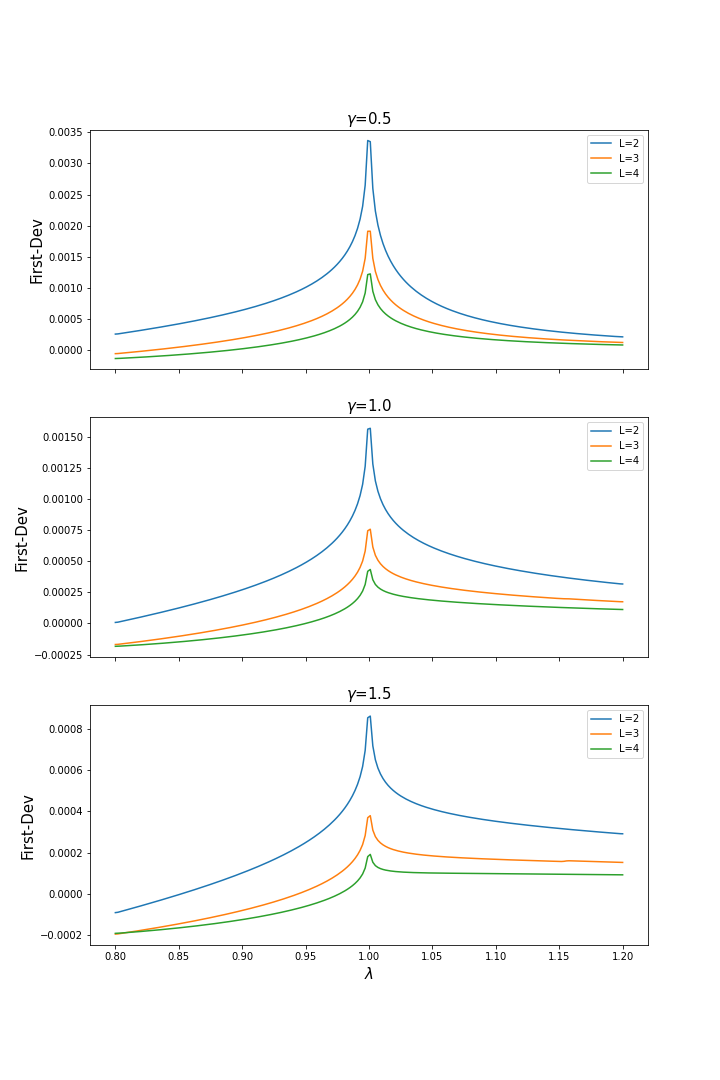
\includegraphics[width=\linewidth]{graphs/firstdev_234_3gammas}
	\caption{Analitical First-Derivative-Max-Ergotropy}
	\label{fig:first2343gammas}
\end{figure}

\begin{figure}
	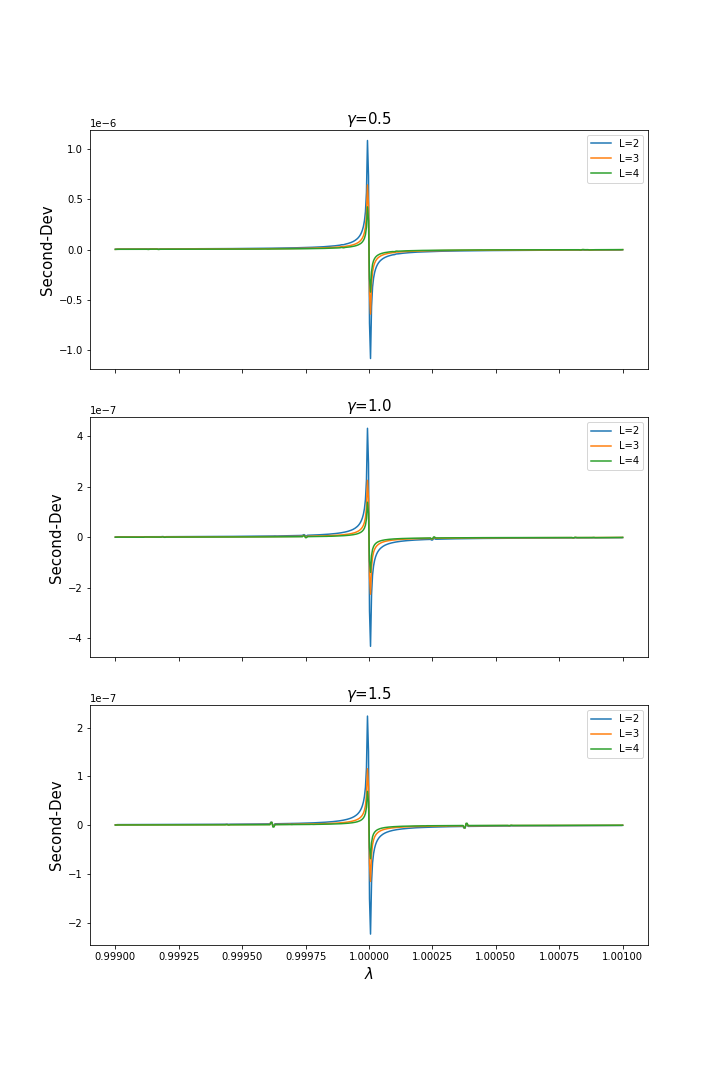
\includegraphics[width=\linewidth]{graphs/Seconddev_234_3gammas}
	\caption{Analitical Second-Derivative-Max-Ergotropy}
	\label{fig:seconddev2343gammas}
\end{figure}






\clearpage
\chapter{Numerical Simulations}
For simulations on two distant sites, it's difficult to access the wavefunction directly, but we can calculate the 8 correlators :

The Hamiltonian \ref{eq:XYmodel} has a symmetry:
\begin{equation}\label{eq:symm}\left(\prod_{l} \sigma_{l}^{z}\right) H\left(\prod_{l} \sigma_{l}^{z}\right)=H\end{equation}
That allows us to say that:
\begin{equation}\rho_{\mu_{1}\cdots  \mu_{L}}=\left\langle\sigma_{1}^{\mu_{1}}\cdots  \sigma_{L}^{\mu_{L}}\right\rangle=0 \quad \text{if the sum of $\mu=x$ and $\mu=y$ is odd}\end{equation}
For example in our case ($L=2$): $\rho_{x0}=\rho_{zy}=0$ \\
The only non-vanishing terms are:
\begin{equation}
	\rho_{00}\quad \rho_{xx} \quad \rho_{yy} \quad \rho_{xy} \quad \rho_{yx} \quad \rho_{zz}
	\quad \rho_{z0} \quad \rho_{0z}
\end{equation}
This could be interesting to understand the "range of correlations".

To simulate the Symmetry Breaking mechanism, we add a little magnetic field in the X direction, we distinguish between the "preserved symmetry" and "broken symmetry" simulations.

\section{Preserved Symmetry}


\begin{figure}[h]
	\centering
	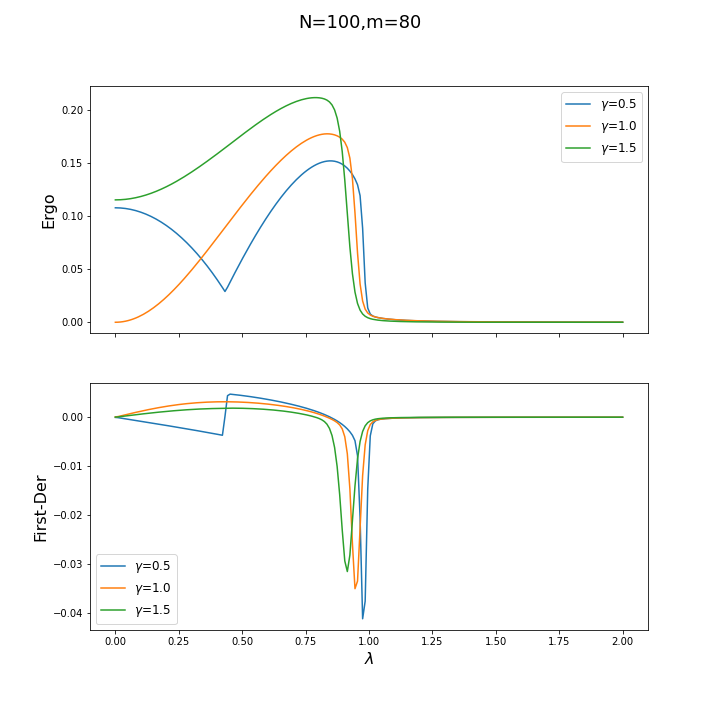
\includegraphics[width=0.7\linewidth]{graphs/N100_m80_pressym_g_051015}
	\caption{Dmrg with preserved Symmetry, 100 sites, 80 states kept.}
	\label{fig:n100m80pressymg051015}
\end{figure}





\begin{figure}[h]
	\centering
	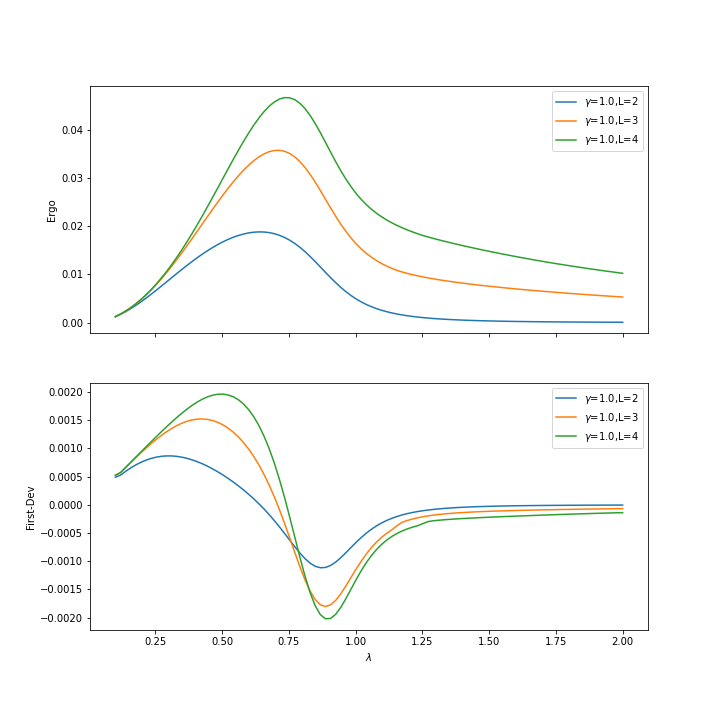
\includegraphics[width=0.7\linewidth]{graphs/ergo_lanczos}
	\caption{Two to four site Ergotropy, $E(\rho)$ and $E(pas)$, Lanczos 12 sites}
	\label{fig:ergolanczos}
\end{figure}


\clearpage
\section{Broken Symmetry}

The factorizing field is found to be: $\lambda_f= \frac{\sqrt{(1-\gamma^2)}}{2}$ \\
\begin{figure}[h]
	\centering
	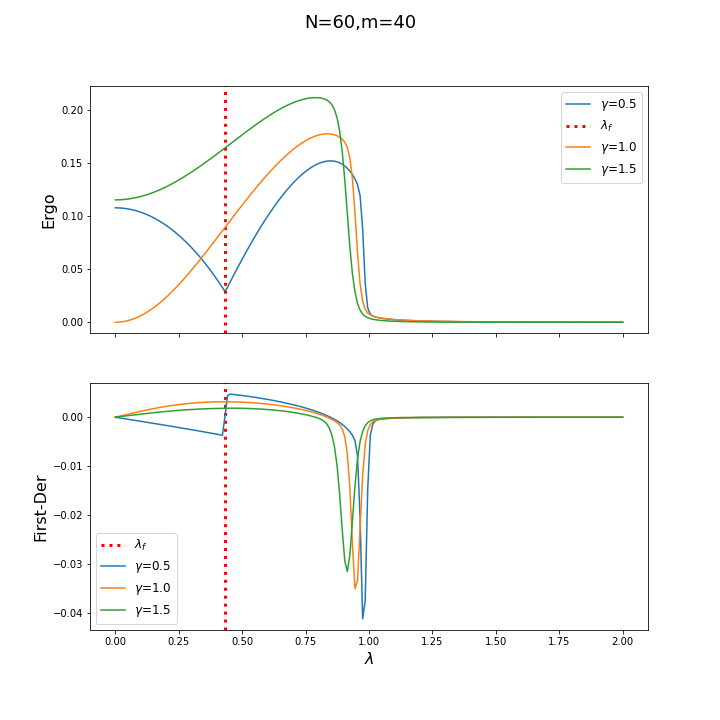
\includegraphics[width=0.7\linewidth]{graphs/N60_m40_simbreak_g_051015}
	\caption{Two-site Ergotropy. Dmrg simulation on 60 sites and 40 states kept. Finite-size effects are visible. The factorization point leads to a non analyticity in the first-der. }
	\label{fig:n60m40simbreakg051015}
\end{figure}

\begin{figure}[h]
	\centering
	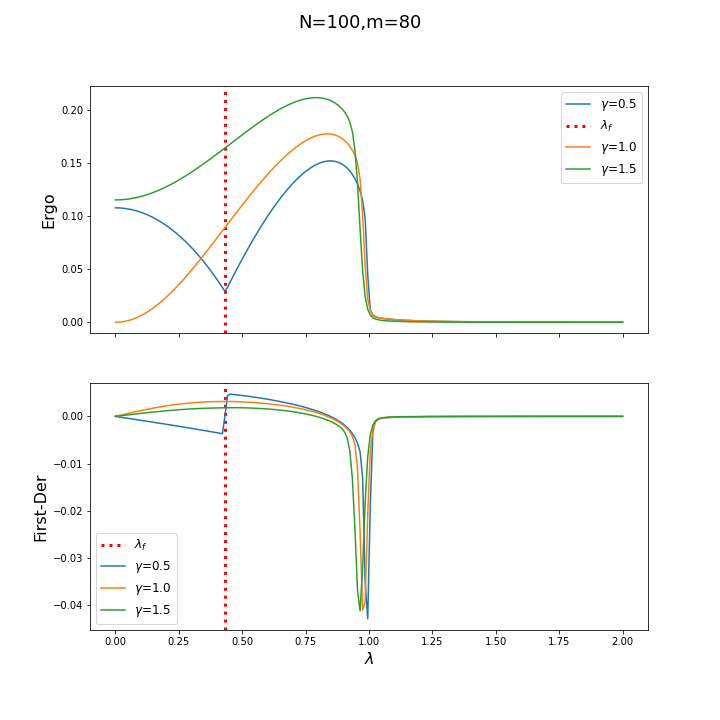
\includegraphics[width=0.7\linewidth]{graphs/N100_m80_simbreak_g_051015}
	\caption{}
	\label{fig:n100m80simbreakg051015}
\end{figure}

\begin{figure}[h]
	\centering
	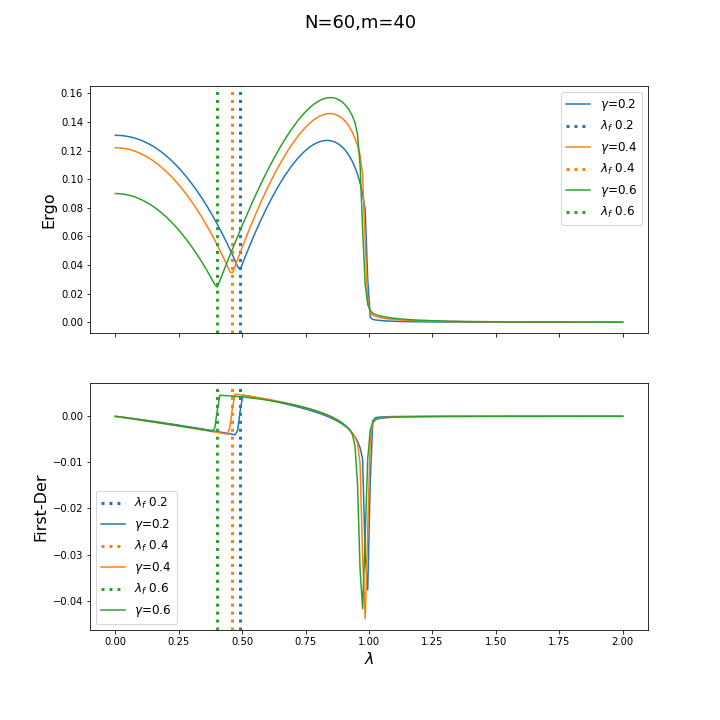
\includegraphics[width=0.7\linewidth]{graphs/N60_m40_simbreak_g_020406}
	\caption{}
	\label{fig:n60m40simbreakg020406}
\end{figure}

\begin{figure}[h]
	\centering
	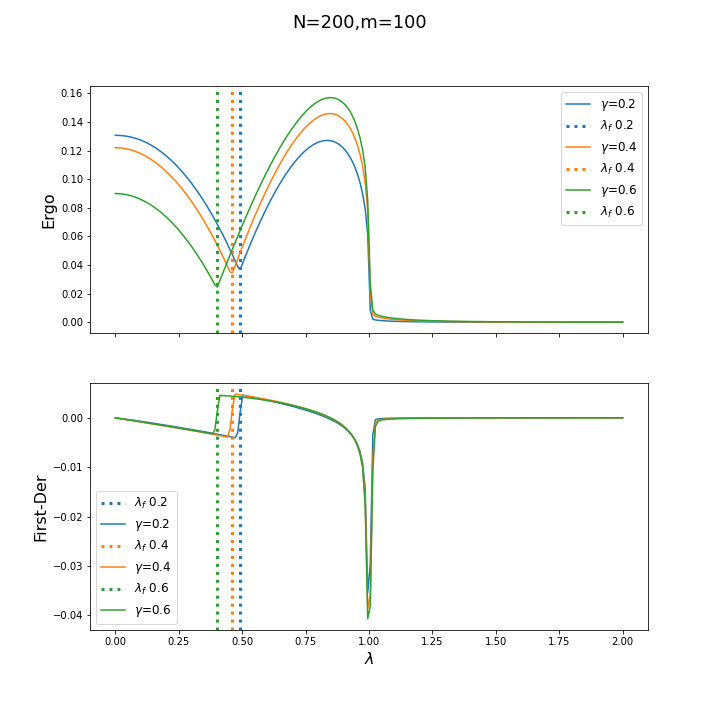
\includegraphics[width=0.7\linewidth]{graphs/N200_m100_simbreak_g_020406}
	\caption{Here we can see that the finite-size effect are negligible. }
	\label{fig:n200m100simbreakg020406}
\end{figure}

\chapter{Conclusions}
conclusions
\clearpage
\appendix
\chapter{Correlation Matrix derivation}\label{appendixcalculation}
We switch to the momentum representation to exploit the translational symmetry with the help of 2N auxiliary Majorana operators:
\begin{equation}\label{eq:ddefinition}\left[\begin{array}{c}
		\check{d}_{2 k-1} \\
		\check{d}_{2 k}
	\end{array}\right]=\sqrt{\frac{2}{N}} \sum_{l=-\frac{N-1}{2}}^{\frac{N-1}{2}} \cos \frac{2 \pi k l}{N}\left[\begin{array}{c}
		\check{a}_{2 l-1} \\
		\check{a}_{2 l}
	\end{array}\right]\end{equation}

\begin{equation}\label{eq:edefinition}\left[\begin{array}{c}
		\check{e}_{2 k-1} \\
		\check{e}_{2 k}
	\end{array}\right]=\sqrt{\frac{2}{N}} \sum_{l=-\frac{N-1}{2}}^{\frac{N-1}{2}} \sin \frac{2 \pi k l}{N}\left[\begin{array}{c}
		\check{a}_{2 l-1} \\
		\check{a}_{2 l}
	\end{array}\right]\end{equation}	
With $0\le k \le N/2$. \\
\begin{equation}\begin{aligned}
		&\check{d}_{k}^{\dagger}=\check{d}_{k}, \quad\left\{\check{d}_{k}, \check{d}_{q}\right\}=\delta_{k q}\\
		&\check{e}_{k}^{\dagger}=\check{e}_{k}, \quad\left\{\check{e}_{k}, \check{e}_{q}\right\}=\delta_{k q}\\
	\end{aligned}	
\end{equation} \\ 
Using the inverse relations:
\begin{equation}\left[\begin{array}{c}
		\check{a}_{2 l-1} \\
		\check{a}_{2 l}
	\end{array}\right]=\sqrt{\frac{2}{N}} \sum_{k=0}^{N/2} e^{-\frac{2 \pi i k l}{N}}\left[\begin{array}{c}
		\check{d}_{2 k-1}+i\check{e}_{2 k-1} \\
		\check{d}_{2 k}+i\check{e}_{2 k}
	\end{array}\right]
\end{equation}


Substituting in \ref{eq:hamiltwitha}:
\begin{equation}\begin{aligned}
		&H =\frac{i}{2} \sum_{l=-\frac{N-1}{2}}^{\frac{N-1}{2}} \check{a}_{2 l} \check{a}_{2 l+1}  
		+ \lambda \check{a}_{2 l-1} \check{a}_{2 l} \\
		&=\frac{i}{2}\sum_{l=-\frac{N-1}{2}}^{\frac{N-1}{2}} \frac{2}{N}\sum_{k_1=0}^{N/2} e^{\frac{2 \pi i k_1 l}{N}}   \left(\check{d}_{2 k_1}-i\check{e}_{2 k_1}\right) \sum_{k_2=0}^{N/2} e^{\frac{-2 \pi i k_2 (l+1)}{N}}  \left(\check{d}_{2 k_2-1}+i\check{e}_{2 k_2-1}  \right)  \\
		&-\lambda\frac{i}{2} \frac{2}{N}\sum_{k_3=0}^{N/2} e^{\frac{2 \pi i k_3 l}{N}}   \left(\check{d}_{2 k_3}-i\check{e}_{2 k_3}\right) \sum_{k_4=0}^{N/2} e^{\frac{-2 \pi i k_4 l}{N}}  \left(\check{d}_{2 k_4-1}+i\check{e}_{2 k_4-1}  \right)\end{aligned}
\end{equation}	
Summing on $l$ first and noting that:
\begin{equation}\label{eq:delta}\begin{aligned}
		&\frac{1}{N}\sum_{l=-\frac{N-1}{2}}^{\frac{N-1}{2}}e^{\frac{2 \pi i (k_1-k_2) l}{N}} = \delta_{k_1,k_2}\\
	\end{aligned}
\end{equation}
we obtain:

\begin{equation}H=\sum_{k=0}^{N / 2} H_{k} \end{equation}
with:
\begin{equation}
	H_k =i   \left(e^{-\frac{2\pi i k}{N}} 
	- \lambda \right)  \left(\check{d}_{2 k}-i\check{e}_{2 k}\right) \left(\check{d}_{2 k-1}+i\check{e}_{2 k-1}  \right)
\end{equation}
\begin{equation}
	H_k =i  \left(\cos \frac{2 \pi k }{N}-i\sin \frac{2 \pi k }{N}
	- \lambda \right)  \left(\check{d}_{2 k}\check{d}_{2 k-1}+\check{e}_{2 k}\check{e}_{2 k-1}-i\check{e}_{2k}\check{d}_{2k-1}+i\check{d}_{2k}\check{e}_{2k-1}\right) 
\end{equation}

\begin{equation}H_{k}=\frac{i\Lambda_k}{2}\left[\begin{array}{c}
		\check{d}_{2 k-1} \\
		\check{e}_{2 k-1} \\
		\check{d}_{2 k} \\
		\check{e}_{2 k}
	\end{array}\right]^{T}\left[\begin{array}{cccc}
		0 & 0 & c_{k} & -s_{k} \\
		0 & 0 & s_{k} & c_{k} \\
		-c_{k} &-s_{k} & 0 & 0 \\
		s_{k} &- c_{k} & 0 & 0
	\end{array}\right]\left[\begin{array}{c}
		\check{d}_{2 k-1} \\
		\check{e}_{2 k-1} \\
		\check{d}_{2 k} \\
		\check{e}_{2 k}
	\end{array}\right]\end{equation}
\newline
\begin{equation}
	\begin{aligned}
		&\Lambda_k \equiv\sqrt{\left(\cos \frac{2 \pi k }{N}-\lambda\right)^2+\sin^2 \frac{2 \pi k }{N}}
		\\
		&c_{k}\equiv\left(\lambda-\cos \frac{2 \pi k }{N}\right)/\Lambda_k
		\\
		&s_{k}\equiv\left(-\sin \frac{2 \pi k }{N}\right)/\Lambda_k
	\end{aligned}
\end{equation}\\
Since by construction $c_k^2+s_k^2=1$,
$\left[\begin{array}{cccc}
	0 & 0 & c_{k} & -s_{k} \\
	0 & 0 & s_{k} & c_{k} \\
	-c_{k} &-s_{k} & 0 & 0 \\
	s_{k} &- c_{k} & 0 & 0\end{array}\right]^2 =-I$ \\
So it exist an orthogonal transformation that defines new operators $\check{b}_{p},  -N\le p \le N-1$ :

\begin{equation}\label{eq:orthogonal}\left[\begin{array}{c}
		\check{b}_{-2 k-1} \\
		\check{b}_{-2 k} \\
		\check{b}_{2 k-1} \\
		\check{b}_{2 k}
	\end{array}\right]=\frac{1}{\sqrt{2}}\left[\begin{array}{cccc}
		u_{k} & v_{k} & u_{k} & -v_{k} \\
		u_{k} & v_{k} & -u_{k} & v_{k} \\
		v_{k} & -u_{k} & v_{k} & u_{k} \\
		-v_{k} & u_{k} & v_{k} & u_{k}
	\end{array}\right]\left[\begin{array}{c}
		\check{d}_{2 k-1} \\
		\check{e}_{2 k-1} \\
		\check{d}_{2 k} \\
		\check{e}_{2 k}
	\end{array}\right]\end{equation}	
and puts the Hamiltonian in the block diagonal form (canonical form for a skew-symmetric matrix):
\begin{equation}H=\frac{i}{2} \sum_{k=-\frac{N-1}{2}}^{\frac{N-1}{2}} \Lambda_k\left(\tilde{b}_{2 k-1} \tilde{b}_{2 k}-\tilde{b}_{2 k} \tilde{b}_{2 k-1}\right)=
	\frac{i}{2}\bigoplus_{k=-\frac{N-1}{2}}^{\frac{N-1}{2}} \Lambda_k\left[\begin{array}{cc}
		0 & 1 \\
		-1 & 0
	\end{array}\right]\end{equation}	
For one moment we switch to non-Hermitian fermionic operators:
\begin{equation}\hat{b}_{k} \equiv \frac{\check{b}_{2 k-1}+i \check{b}_{2 k}}{2}\end{equation}
\begin{equation}
	H= \sum_{k=-\frac{N-1}{2}}^{\frac{N-1}{2}} \Lambda_k\hat{b}_k^\dagger\hat{b}_k-\Lambda_k/2
\end{equation}
The second term is a constant and can be ignored.\\
Now since all $\Lambda_k>0$ we can finally find the ground state imposing
$b_k\ket{ \psi_g}=0$ \\ From which also: $\hat{b}_k^\dagger \hat{b}_k\ket{ \psi_g}=\hat{b}_k \hat{b}_k\ket{ \psi_g}=0$ and  $b_k \hat{b}_k^\dagger\ket{\psi_g}=\ket{\psi_g}$ \\
Using as always the inverse transformations we can calculate the correlation matrix on the ground state for the Majorana operators:
\begin{equation}\begin{split}
		&<\check{b}_{2k-1}\check{b}_{2k}>=i<\hat{b}_k\hat{b}_k^\dagger>=i\\ &<\check{b}_{2k}\check{b}_{2k-1}>=-i<\hat{b}_k\hat{b}_k^\dagger>=-i \\&<\check{b}_{2k}\check{b}_{2k}>=<\check{b}_{2k-1}\check{b}_{2k-1}>=<\hat{b}_k\hat{b}_k^\dagger>=1\\
	\end{split}
\end{equation}\\
In compact notation:
\begin{equation}
	\left\langle\check{b}_{p} \check{b}_{q}\right\rangle=\delta_{p q}+i \Gamma_{p q}^{B}
\end{equation}

\begin{equation}\label{eq:corrmatrb}\Gamma^{B}=\bigoplus_{k=-\frac{N-1}{2}}^{\frac{N-1}{2}}\left[\begin{array}{rr}
		0 & 1 \\
		-1 & 0
	\end{array}\right]\end{equation}
Now that we have the correlation matrix for the $\check{b}$ operators we have to go back to the $\check{a}$, that means we have to find the matrix $W$:
\begin{equation}\label{eq:wmatrix}\check{b}_{p}=\sum_{m=-N}^{N-1} W_{p m} \check{a}_{m}, \quad-N+1 \leq p \leq N\end{equation}
The orthogonal transformation that defines the $\check{b}$ operators:
\begin{equation}\label{eq:orthogonal2}\left[\begin{array}{c}
		\check{b}_{-2 k-1} \\
		\check{b}_{-2 k} \\
		\check{b}_{2 k-1} \\
		\check{b}_{2 k}
	\end{array}\right]=\frac{1}{\sqrt{2}}\left[\begin{array}{cccc}
		u_{k} & v_{k} & u_{k} & -v_{k} \\
		u_{k} & v_{k} & -u_{k} & v_{k} \\
		v_{k} & -u_{k} & v_{k} & u_{k} \\
		-v_{k} & u_{k} & v_{k} & u_{k}
	\end{array}\right]\left[\begin{array}{c}
		\check{d}_{2 k-1} \\
		\check{e}_{2 k-1} \\
		\check{d}_{2 k} \\
		\check{e}_{2 k}
	\end{array}\right]\end{equation}
has coefficients $u_k=\cos(\theta_k/2)$, $v_k=\sin(\theta_k/2)$ such that:
\begin{equation}\begin{aligned}
		&u_k^2-v_k^2=\cos(\theta_k)=\left(\lambda-\cos \frac{2 \pi k }{N}\right)/\Lambda_k\\
		&2u_kv_k=\sin(\theta_k)=\left(-\sin \frac{2 \pi k }{N}\right)/\Lambda_k\\
	\end{aligned}
\end{equation} 
For the sake of clarity we split the transformation \ref{eq:orthogonal2} in two even and odd parts:
\begin{equation}\label{eq:orthogonaevenodd}\left[\begin{array}{c}
		\check{b}_{-2 k-1} \\
		\check{b}_{-2 k} \\
		\check{b}_{2 k-1} \\
		\check{b}_{2 k}
	\end{array}\right]=\frac{1}{\sqrt{2}}\left[\begin{array}{cc}
		u_{k} & v_{k}  \\
		u_{k} & v_{k}  \\
		v_{k} & -u_{k} \\
		-v_{k} & u_{k} 
	\end{array}\right]\left[\begin{array}{c}
		\check{d}_{2 k-1} \\
		\check{e}_{2 k-1} 
	\end{array}\right]+\frac{1}{\sqrt{2}}\left[\begin{array}{cc}
		u_{k} & -v_{k}  \\
		-u_{k} & v_{k}  \\
		v_{k} & u_{k} \\
		v_{k} & u_{k} 
	\end{array}\right]\left[\begin{array}{c}
		\check{d}_{2 k} \\
		\check{e}_{2 k} 
	\end{array}\right]\end{equation}\\
and now using the definitions of $\check{d}$ and $\check{e}$ ( \ref{eq:ddefinition} , \ref{eq:edefinition} ):
\begin{equation}\label{eq:orthogonalba}\left[\begin{array}{c}
		\check{b}_{-2 k-1} \\
		\check{b}_{-2 k} \\
		\check{b}_{2 k-1} \\
		\check{b}_{2 k}
	\end{array}\right]=\frac{1}{\sqrt{N}}\sum_{l=-\frac{N-1}{2}}^{\frac{N-1}{2}}\left(\left[\begin{array}{cc}
		u_{k} & v_{k}  \\
		u_{k} & v_{k}  \\
		v_{k} & -u_{k} \\
		-v_{k} & u_{k} 
	\end{array}\right]\left[\begin{array}{c}
		\cos \frac{2 \pi k l}{N}  \\
		\sin \frac{2 \pi k l}{N}  
	\end{array}\right]\check{a}_{2l-1}+
	\left[\begin{array}{cc}
		u_{k} & -v_{k}  \\
		-u_{k} & v_{k}  \\
		v_{k} & u_{k} \\
		v_{k} & u_{k} 
	\end{array}\right]\left[\begin{array}{c}
		\cos \frac{2 \pi k l}{N}  \\
		\sin \frac{2 \pi k l}{N}  
	\end{array}\right]\check{a}_{2l}\right) \end{equation}
With this equation \ref{eq:orthogonalba} we can read the coefficients of $W$ as defined in \ref{eq:wmatrix}.
\newline
The correlation matrix $\Gamma^A$ for the operators $\check{a}$ is given by:
\begin{equation}
	\Gamma^A=W^T\Gamma^BW
\end{equation}
Using the definition of $\Gamma^B$ \ref{eq:corrmatrb}:
\begin{equation}\label{eq:corrmatra}
	\Gamma^A_{mn}= \sum_{i,j}  W^T_{mi} \Gamma^B_{ij} W_{jn}=\sum_{k=-\frac{N-1}{2}}^{\frac{N-1}{2}} W^T_{m , 2k-1}W_{2k,n}-W^T_{m , 2k}W_{2k-1,n}=\sum_{k=-\frac{N-1}{2}}^{\frac{N-1}{2}}  W_{2k-1,m}W_{2k,n}-W_{2k , m}W_{2k-1,n}
\end{equation}\\
Now using \ref{eq:orthogonalba} and \ref{eq:corrmatra} we explicitly calculate an element of the correlation $\Gamma^A$ :
\begin{equation}\begin{aligned}\label{eq:finiten}
		&<\check{a}_{2m-1}\check{a}_{2n}>=\Gamma^A_{2m-1,2n}=\sum_{k=-\frac{N-1}{2}}^{\frac{N-1}{2}}  W_{2k-1,2m-1}W_{2k,2n}-W_{2k , 2m-1}W_{2k-1,2n}=\\
		&\sum_{k=1}^{\frac{N-1}{2}}\left(  W_{2k-1,2m-1}W_{2k,2n}-W_{2k , 2m-1}W_{2k-1,2n}+W_{-2k-1,2m-1}W_{-2k,2n}-W_{-2k , 2m-1}W_{-2k-1,2n}\right)+ \\&W_{-1,2m-1}W_{0,2n}-W_{-1 , 2m-1}W_{0,2n}=\\
		&=\frac{2}{N}\sum_{k=1}^{\frac{N-1}{2}}\left(v_k \cos \frac{2 \pi k m}{N}-u_k\sin \frac{2 \pi k m}{N}\right)\left(v_k\cos \frac{2 \pi k n}{N}+u_k\sin \frac{2 \pi k n}{N}\right)+\\& \left(u_k \cos \frac{2 \pi k m}{N}+v_k\sin \frac{2 \pi k m}{N}\right)\left(v_k\sin \frac{2 \pi k n}{N}-u_k\cos \frac{2 \pi k n}{N}\right)-u_0^2= \\
		&\frac{2}{N}\sum_{k=0}^{\frac{N}{2}}\cos(\theta_k)\cos{\frac{2\pi k (m-n)}{N}}-\sin(\theta_k)\sin{\frac{2\pi k (m-n)}{N}}\\\\
	\end{aligned}	
\end{equation}
Now calling $\phi \equiv \frac{2\pi k}{N}$ and sending $N\rightarrow\infty$:
\begin{equation}
	<\check{a}_{2m-1}\check{a}_{2n}>=\frac{1}{\pi}\int_{0}^{\pi}d\phi    \frac{\lambda-\cos\phi}{|\lambda-\cos\phi+i\sin\phi|}\cos{\phi(m-n)}-\frac{1}{\pi}\int_{0}^{\pi}d\phi \frac{\sin\phi}{|\lambda-\cos\phi+i\sin\phi|}\sin{\phi(m-n)}
\end{equation}
Wich can be written in the more compact form:
\begin{equation}
	<\check{a}_{2m-1}\check{a}_{2n}>=\frac{1}{2\pi}\int_{0}^{2\pi}d\phi \  e^{-i \phi  (n-m)} \frac{\lambda-\cos\phi+i\sin\phi}{|\lambda-\cos\phi+i\sin\phi|}
\end{equation}

\bibliographystyle{alpha}
\bibliography{ergo_thesis_bib}

\end{document}
